\documentclass[journal]{IEEEtran}
\usepackage[T1]{fontenc}
\usepackage{amsmath,amssymb}
\usepackage{graphicx}
\usepackage{booktabs,array}
\usepackage{cite}
\usepackage[hidelinks]{hyperref}
\newcommand{\dd}{\mathrm{d}}
\newcommand{\etal}{\eta_{\mathrm{tot}}}
\newcommand{\etam}{\eta_{\mathrm{mode}}}
\newcommand{\Topt}{T_{\mathrm{opt}}}
\newcommand{\SNU}{\mathrm{SNU}}
\newcommand{\F}{\mathcal{F}}
\hyphenation{Torch-Optics Straw-berry Fields}
\begin{document}
\raggedbottom
\title{Fourier-Domain Spatial-Mode Conditioning for Coherent Optical Communication: A Reproducible Numerical Study}
\author{Afam Madu and Tofayel Karim}
\maketitle

\begin{abstract}
Spatial-mode mismatch reduces the signal collected by a coherent receiver even when an optical field retains nearly all of its power. We investigate phase-only Fourier-plane conditioning in an ideal sampled scalar paraxial relay, separating optical throughput, normalized local-oscillator overlap, and quantum-limited homodyne statistics. A differentiable phase mask is trained on displaced, tilted, defocused, and astigmatic Gaussian fields and selected using independent validation data. On 24 held-out distortions, mean overlap is 0.431225 without correction, 0.469958 with fixed analytic phase alignment, and 0.470226 with the trained mask. The paired trained-minus-uncorrected improvement is 0.039001, with a 95\% Student-$t$ interval of [0.035802, 0.042199]; the corresponding interval relative to analytic correction includes zero. Thus, correction is supported for the tested distribution, but superiority of optimization is not demonstrated. Independent optical references, objective-gradient checks, 41 archived automated tests, and an executed Strawberry Fields Gaussian backend establish consistency with the stated numerical models. Pure-loss validation preserves coherent-state variance at one shot-noise unit. A deliberately occluded and attenuated field has throughput 0.061736 and a tight phase-only overlap ceiling of 0.243860, demonstrating a limitation that cannot be overcome by further phase optimization. All results are simulations: no experiment, fabricated device, squeezing, or secret-key rate is claimed.
\end{abstract}
\begin{IEEEkeywords}
Fourier optics, spatial-mode matching, phase-only modulation, coherent communication, homodyne detection, Gaussian quantum states, reproducible simulation.
\end{IEEEkeywords}

\section{Introduction}
\IEEEPARstart{C}{oherent} optical reception is a mode-selective measurement. The receiver does not collect useful coherent signal merely because optical power reaches its entrance plane: the field must also overlap the spatial and phase reference defined by the local oscillator (LO). Misalignment and aberration can therefore reduce the measured signal without comparable attenuation of the total optical field. Fourier-domain phase conditioning provides a direct way to modify this projection, but it does not supply optical gain, invert arbitrary amplitude damage, or change the intrinsic vacuum noise of a coherent state.

This distinction motivates a carefully bounded question: can a single fixed phase-only Fourier mask improve LO coupling over a specified distribution of distorted Gaussian inputs, and what benefit remains when compared with a physically informed analytic mask? The study treats that question as an optical optimization problem followed by a Gaussian receiver model. It does not treat a classical complex field as a complete multimode quantum simulation. Fourier propagation supplies the coupling efficiency; passive-loss Gaussian transformations and independent noise sampling supply the receiver statistics.

The foundations are standard Fourier optics and Gaussian quantum optics \cite{goodman,weedbrook}. The purpose here is not to propose a new Fourier transform, optimization algorithm, or security protocol. Rather, it is to provide an inspectable numerical chain from sampled fields to receiver statistics, with an analytic comparator, held-out evaluation, and explicit failure conditions. A meaningful positive result must survive more than a visually improved intensity map. It must preserve physical normalization, separate training from evaluation, distinguish received signal from vacuum noise, and acknowledge what an ideal phase-only element cannot achieve.

The contributions are fourfold. First, the implementation maintains physical sampling and separates normalized overlap from throughput throughout the propagation and detection calculations. Second, a train/validation/test comparison quantifies the improvement of fixed phase correction without asserting an unsupported advantage of numerical optimization. Third, independent numerical and backend checks document the boundary between verified computation and unverified apparatus assumptions. Fourth, an attainable spectral-magnitude bound establishes why an occlusion-and-attenuation failure case cannot be repaired even by a better phase mask.

The remainder develops the optical model and its bound, describes optimization and sampling, presents the archived correction results, verifies the quantum-noise interface before interpreting homodyne performance, and discusses reproducibility and limitations. Every numerical result and figure is drawn from the existing archived baseline; no additional simulations are introduced for this manuscript.

\section{Optical Model and Physical Normalization}
\subsection{Ideal Focal-Plane Relay}
Figure~\ref{fig:architecture} identifies the classical/quantum boundary. The optical subsystem is an ideal two-dimensional scalar paraxial focal-plane operator. The first transform maps the source field to a Fourier plane, a circular pupil and phase mask modulate that plane, and an inverse transform returns the field to receiver coordinates. Global lens phase and image inversion are absorbed into the coordinate convention. This is not explicit finite-distance propagation through two simulated thin lenses.

\begin{figure*}[!t]
\centering
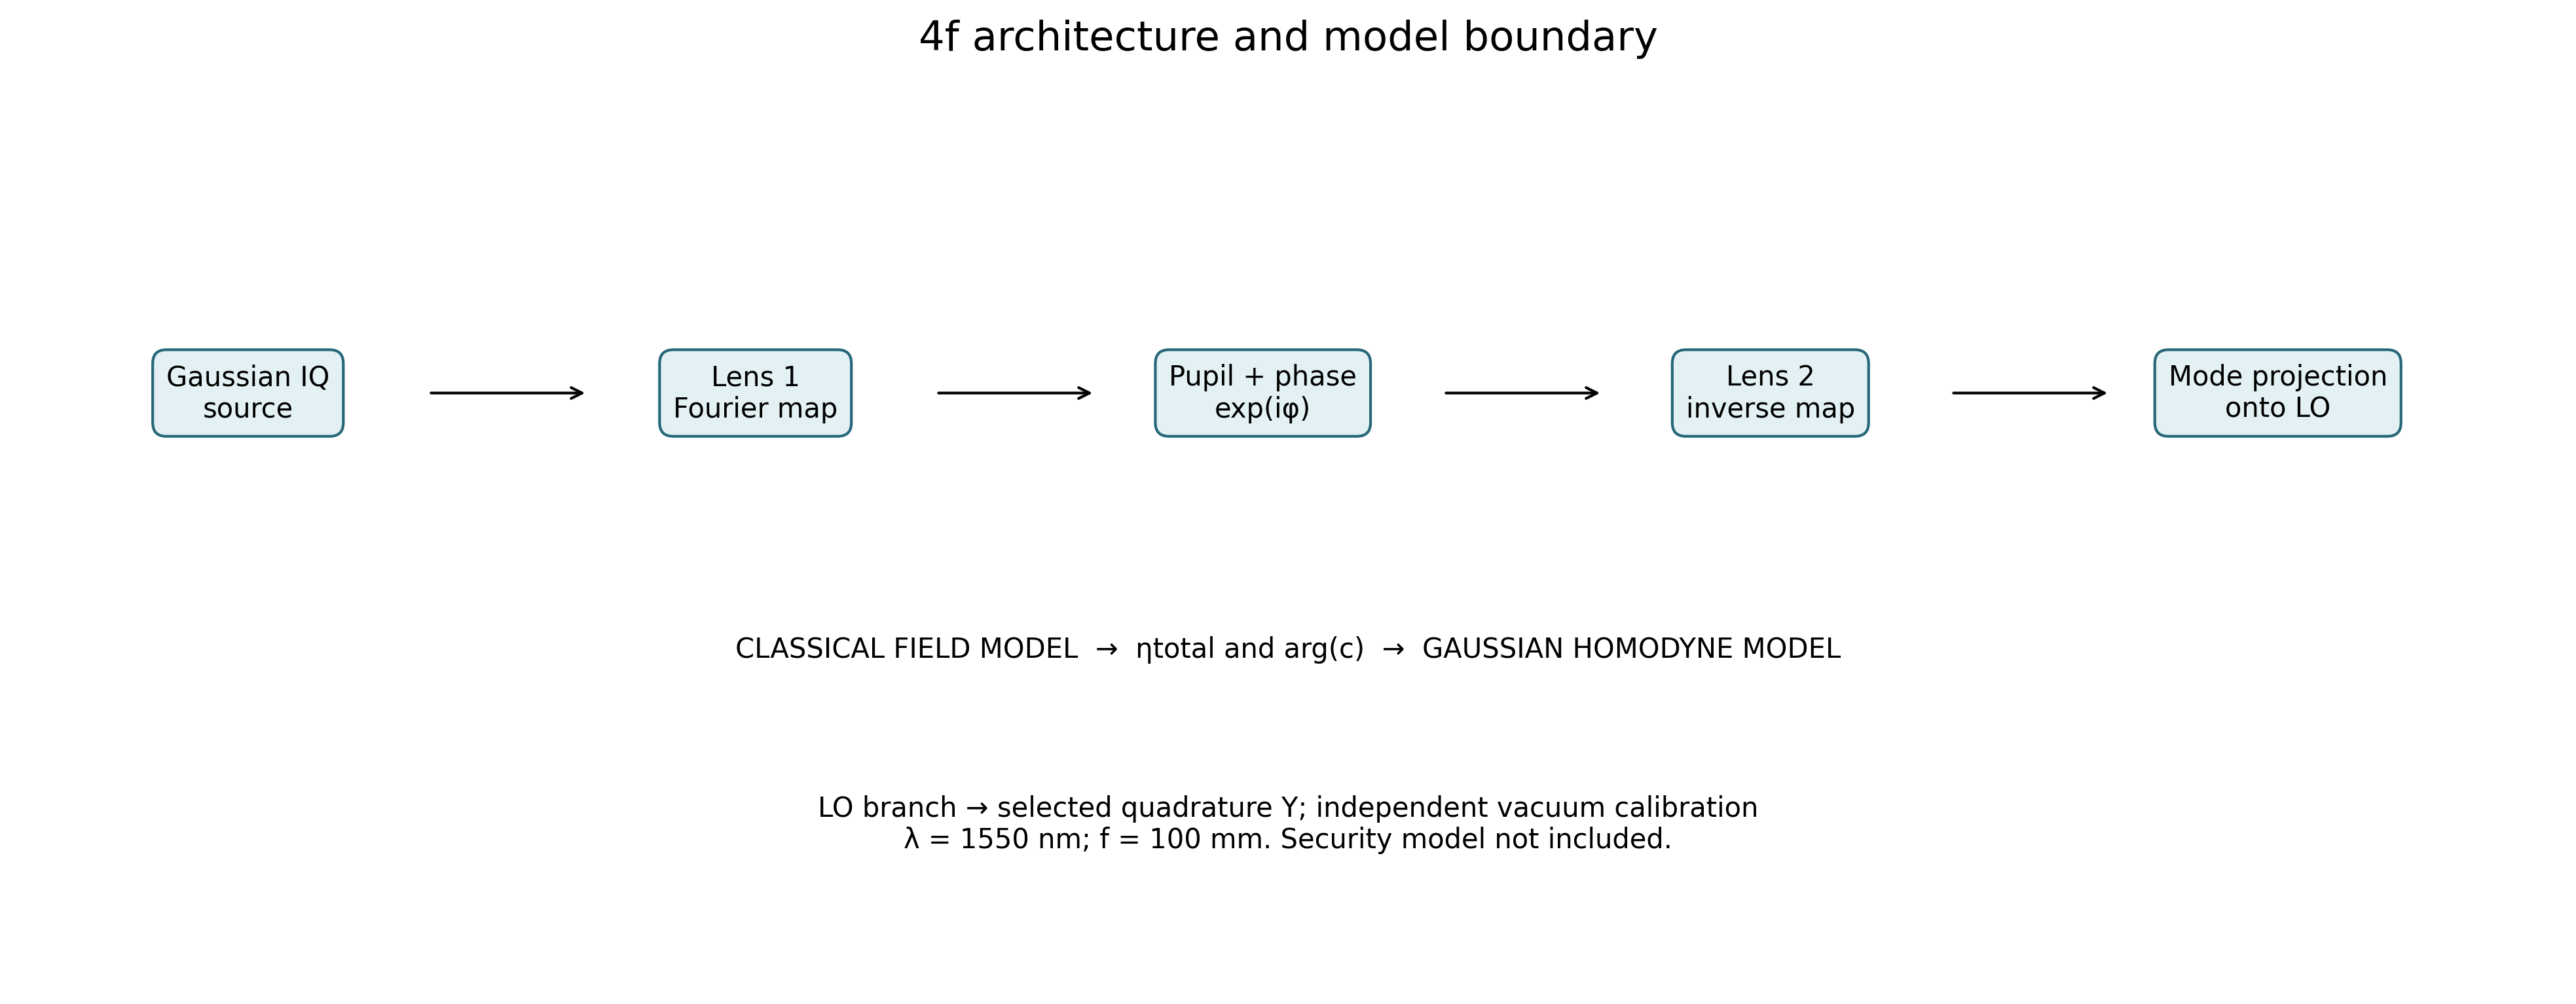
\includegraphics[width=0.96\textwidth]{../results/figures/01_architecture.png}
\caption{Ideal sampled $4f$ operator and the boundary between classical propagation and Gaussian receiver statistics. The Fourier-plane pupil and phase mask determine optical throughput and LO overlap; channel transmission and detector efficiency are applied separately. The drawing is a model schematic, not an experimentally validated lens train. Baseline wavelength is 1550 nm and the transverse grid is $128\times128$.}
\label{fig:architecture}
\end{figure*}

Let $u_{mn}$ be the input field, with transverse pitch $\Delta x$, and let $\F_d$ denote a centered orthonormal two-dimensional discrete Fourier transform. The physical Fourier-plane spacing is
\begin{equation}
 x_F=\lambda f f_x,\qquad \Delta x_F=\frac{\lambda f}{N\Delta x}.
 \label{eq:sampling}
\end{equation}
The field and relay output are implemented as
\begin{align}
 U_F&=\frac{\Delta x}{\Delta x_F}\F_d u,\\
 v&=\frac{\Delta x_F}{\Delta x}\F_d^{-1}\!\left[P e^{i\phi}U_F\right],
 \label{eq:relay}
\end{align}
where $P$ is the real binary circular pupil. The pitch ratio is essential: an orthonormal FFT preserves the unweighted array norm, whereas physical power includes pixel area. Consequently,
\begin{equation}
 \sum_{mn}|U_{F,mn}|^2\Delta x_F^2
 =\sum_{mn}|u_{mn}|^2\Delta x^2.
 \label{eq:power}
\end{equation}
A phase mask has unit modulus and cannot change the Fourier-plane intensity. For this fixed pupil, output power is independent of $\phi$. Any change in collected coherent signal must therefore result from redistribution among spatial modes, not from an increase in total power.

The production path uses complex double-precision Torch tensors, real double-precision phase variables, and the public \texttt{TorchOptics Field.modulate} API at the physical Fourier pitch \cite{torchoptics}. The centered FFT operations use Torch FFT aliases imported from the pinned TorchOptics implementation module. An independent NumPy propagation path supplies reference calculations. Use of the package in production is substantive modulation integration, but is not evidence that the lens train has been modeled with an independent propagation algorithm.

\subsection{Source, Distortions, and Sampled-Window Convention}
The LO is a centered Gaussian with amplitude proportional to $\exp[-(x^2+y^2)/w^2]$. A distorted source is
\begin{align}
 u_{\boldsymbol\theta}(x,y)&=C_{\boldsymbol\theta}
 \exp\!\left[-\frac{(x-d_x)^2+(y-d_y)^2}{w^2}\right]
 e^{i\psi_{\boldsymbol\theta}(x,y)}, \label{eq:source}\\
 \psi_{\boldsymbol\theta}(x,y)&=\frac{2\pi}{\lambda}(\alpha_xx+\alpha_yy)
 +D\frac{x^2+y^2}{w^2}+A\frac{x^2-y^2}{w^2}.
 \label{eq:distortion}
\end{align}
Here $d_x,d_y$ are displacements, $\alpha_x,\alpha_y$ are paraxial tilt angles, and $D,A$ are defocus and astigmatism phase coefficients. In the code the quadratic phases are centered on the grid origin, not translated with the displaced Gaussian. These coefficients are not normalized Zernike coefficients or measured lens prescriptions.

The normalization constant $C_{\boldsymbol\theta}$ is set separately for each sampled Gaussian so that its discrete-window power is unity. Thus displacement of a Gaussian across the numerical window is not itself counted as source aperture loss. This convention defines the modeled input; a finite physical launch aperture would require a separate treatment. The intentional occlusion case introduced later is applied after this normalization, and is not renormalized.

Each distortion parameter is independently normally distributed with the mean and standard deviation in Table~\ref{tab:config}. Samples are untruncated. Independence and normality are simulation assumptions, not conclusions from measured disturbances. Independent pseudorandom seeds generate the training, validation, and test splits.

\begin{table*}[!t]
\caption{Archived Baseline Configuration and Distortion Distribution}
\label{tab:config}
\centering\small
\setlength{\tabcolsep}{4pt}
\begin{tabular}{lll@{\qquad}lll}
\toprule
Optical/numerical setting & Value & Unit & Distortion parameter & Mean & Standard deviation\\
\midrule
Grid & $128\times128$ & samples & $d_x$ & $90~\mu$m & $18~\mu$m\\
Input/output pitch & 12 & $\mu$m & $d_y$ & $-35~\mu$m & $12~\mu$m\\
Wavelength & 1550 & nm & $\alpha_x$ & $0.65$ mrad & $0.10$ mrad\\
Focal length & 100 & mm & $\alpha_y$ & $-0.25$ mrad & $0.08$ mrad\\
Gaussian amplitude radius $w$ & 220 & $\mu$m & $D$ & $1.40$ rad & $0.25$ rad\\
Fourier pupil radius & 3 & mm & $A$ & $0.70$ rad & $0.18$ rad\\
Fourier pitch & 100.911458 & $\mu$m & Distribution & \multicolumn{2}{l}{Independent untruncated normal parameters}\\
\midrule
\multicolumn{3}{l}{Optimization: Adam, learning rate 0.08, 100 updates per initialization} & \multicolumn{3}{l}{Three initializations; seeds 404, 405, 406}\\
\multicolumn{3}{l}{Training/validation/test sizes: 12/12/24} & \multicolumn{3}{l}{Split seeds: 101/202/303}\\
\multicolumn{3}{l}{Channel transmission $T_{\rm ch}=0.8$; detector efficiency $\eta_d=0.9$} & \multicolumn{3}{l}{100,000 homodyne symbols per principal case; seeds 505--509}\\
\multicolumn{3}{l}{Modulation $V_A=4$; receiver excess noise $\xi_{\rm rec}=0.02$} & \multicolumn{3}{l}{Electronic noise $v_{\rm el}=0.01$; phase compensation enabled}\\
\multicolumn{3}{l}{Loss-case neutral intensity transmission: 0.08} & \multicolumn{3}{l}{Half-plane transmission: $x>0$; two Torch CPU threads}\\
\bottomrule
\end{tabular}
\end{table*}

Figure~\ref{fig:fields} shows the physical-plane representation. The Fourier coordinate pitch differs from the source and receiver pitch, although all arrays have the same sample count. Intensities are normalized power densities, expressed in m$^{-2}$, rather than measured irradiances in W/m$^2$. Phase maps suppress pixels below $10^{-6}$ of peak intensity, where a plotted phase would carry little physical meaning. The common linear intensity scaling can also conceal weak spectral structure.

\begin{figure*}[!t]
\centering
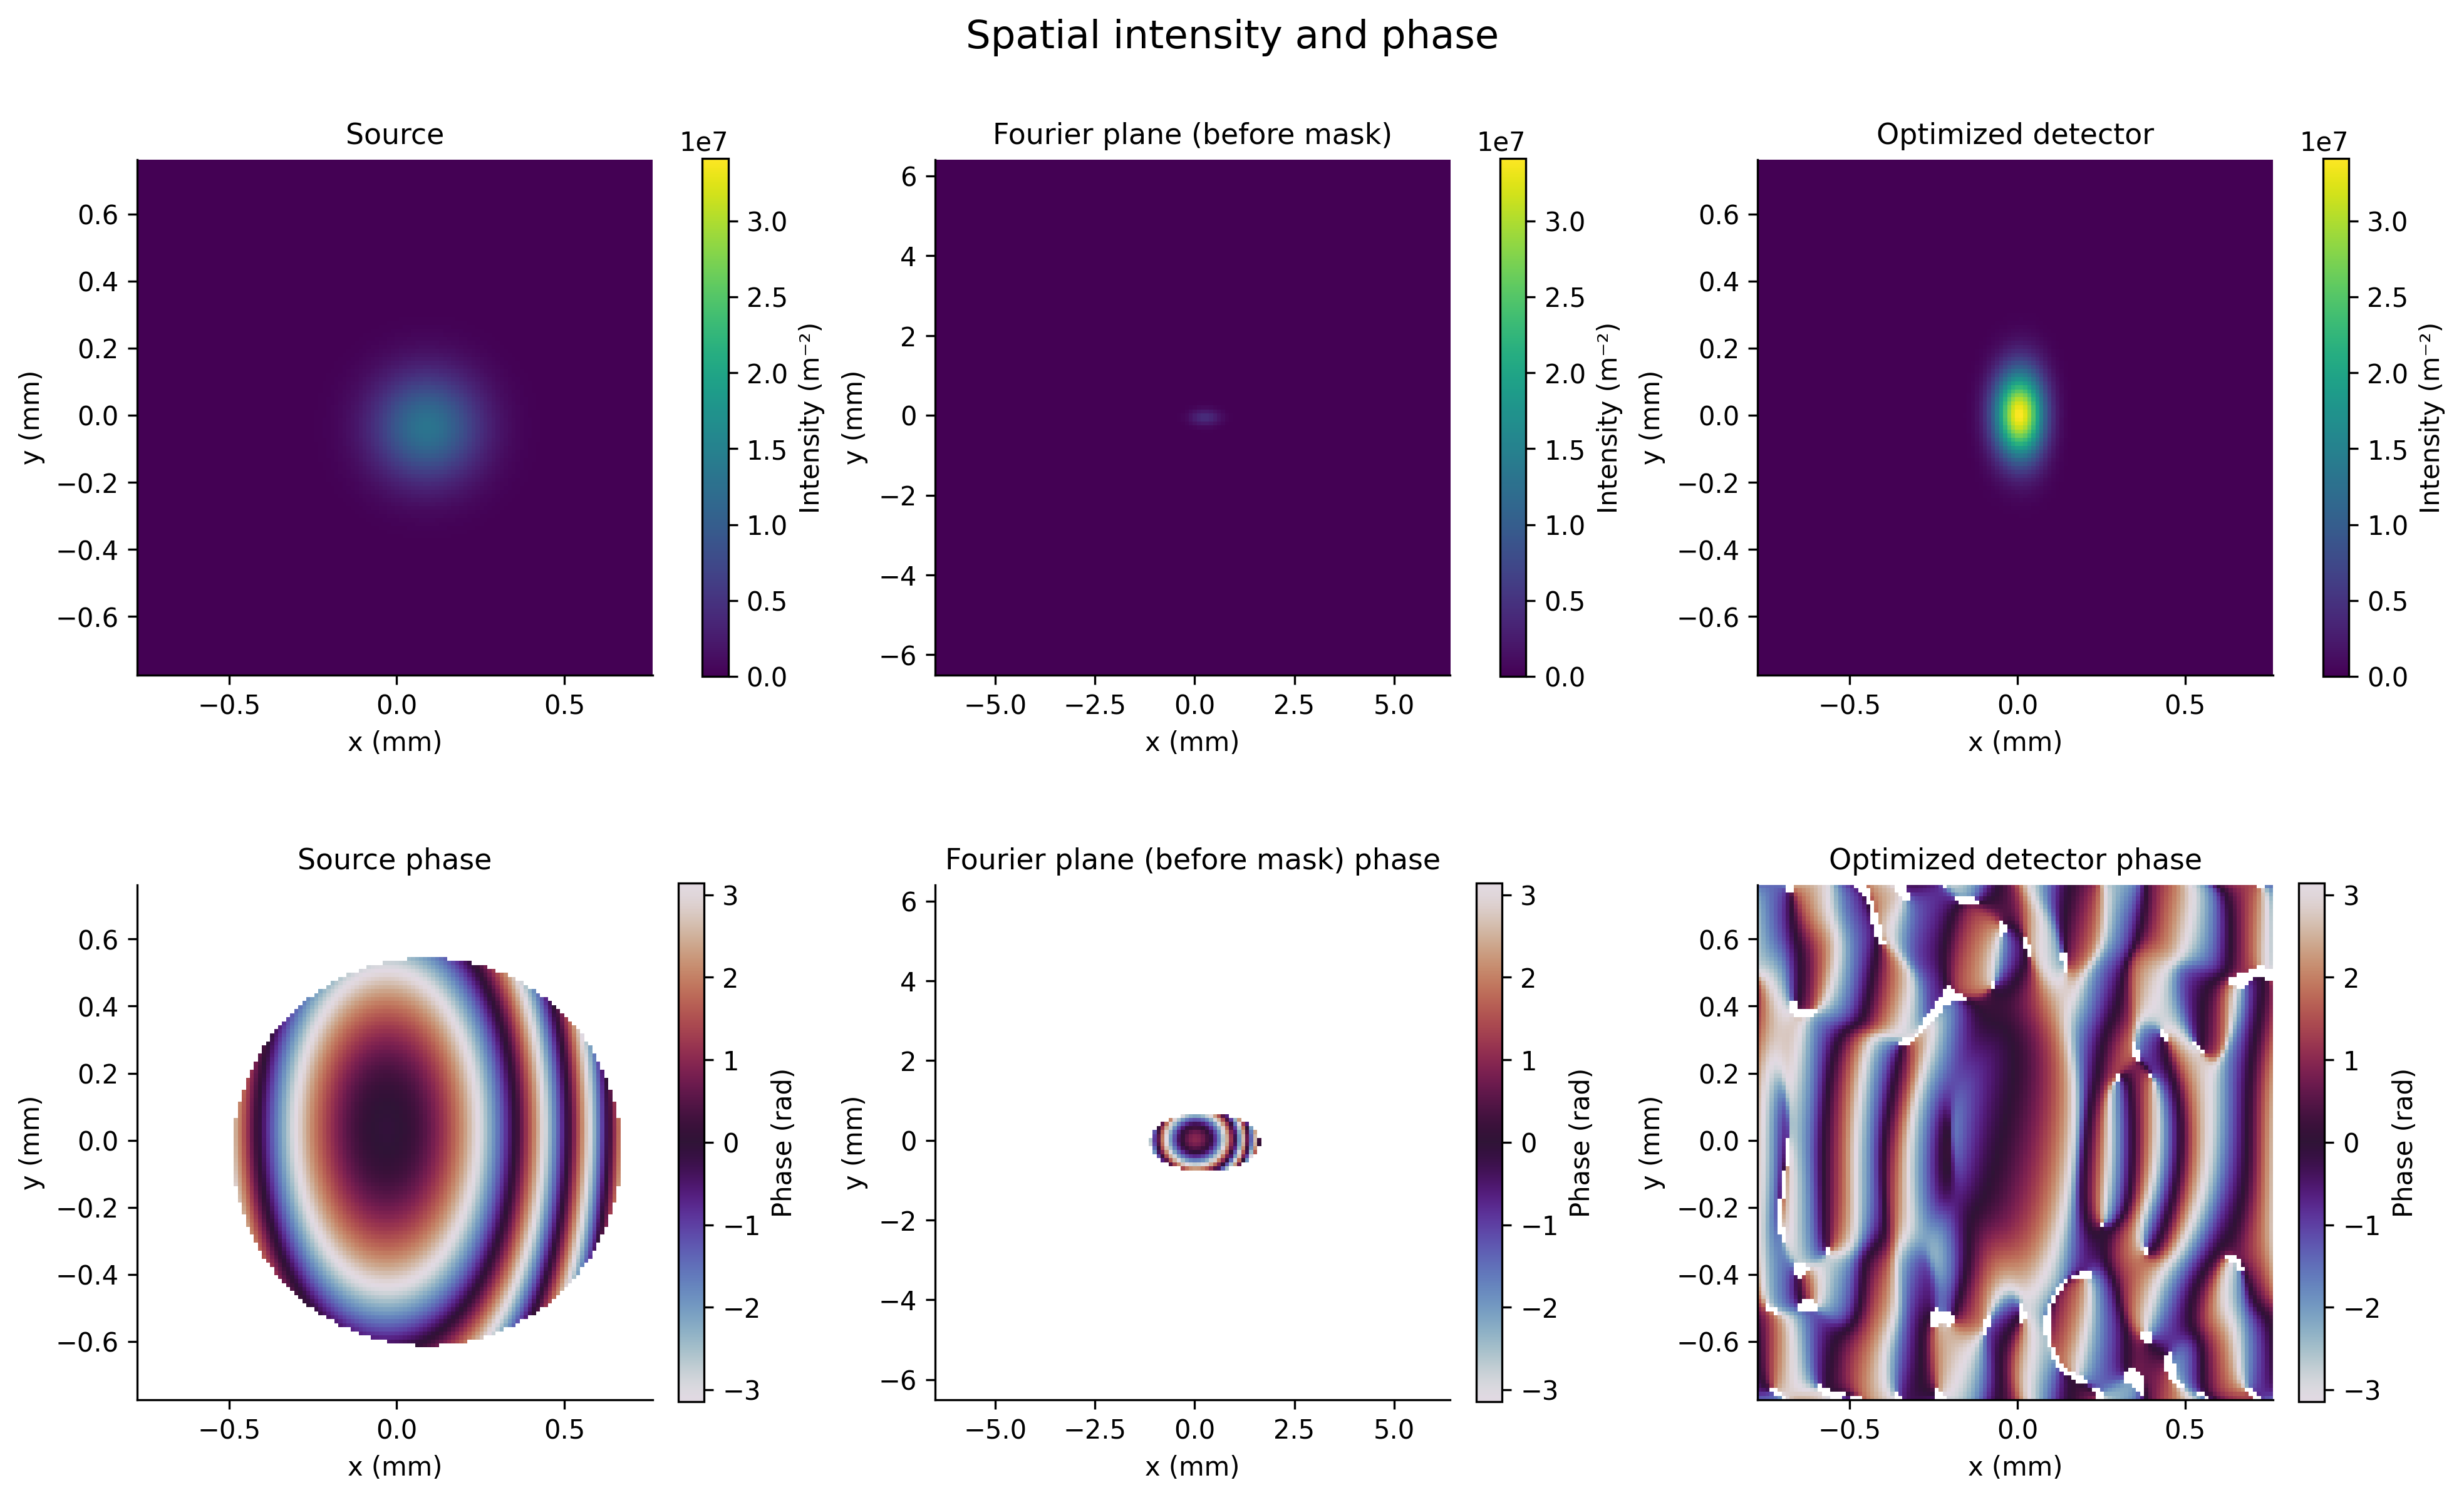
\includegraphics[width=0.98\textwidth]{../results/figures/02_fields.png}
\caption{Source, Fourier-plane, and detector-plane intensity and phase maps for the representative trained-mask case. The Fourier-plane field is shown before the mask/pupil operation, and its physical coordinates follow $x_F=\lambda f f_x$. Integrated source and output powers are unity to numerical accuracy. Intensity units follow the unit-input-power convention; dark phase pixels are suppressed below $10^{-6}$ peak intensity. Equal array size does not imply equal physical pixel area across planes.}
\label{fig:fields}
\end{figure*}

\subsection{Throughput and LO Projection}
For receiver field $v$ and LO mode $\ell$, define
\begin{align}
 P_v&=\sum |v|^2\Delta x^2,\quad
 P_\ell=\sum |\ell|^2\Delta x^2,\\
 c&=\frac{\sum\ell^*v\Delta x^2}{\sqrt{P_\ell P_v}},\quad
 \etam=|c|^2,\quad \Topt=\frac{P_v}{P_{\rm in}}.
 \label{eq:metrics}
\end{align}
The zero-output case is assigned zero overlap. The original input reference is $P_{\rm in}=1$, including for the deliberately attenuated case. The total useful receiver efficiency is
\begin{equation}
 \etal=T_{\rm ch}\Topt\etam\eta_d.
 \label{eq:eta}
\end{equation}
Normalized overlap can remain high even when the output is strongly attenuated; conversely, unit throughput can coexist with substantial mode mismatch. Equation~\eqref{eq:eta} prevents either from being mistaken for complete signal recovery. The overlap phase $\arg c$ is retained for the homodyne reference rather than silently discarded.

\subsection{Analytic Correction and a Tight Phase-Only Bound}
The fixed analytic comparator is formed from the representative source at the distribution mean and the LO:
\begin{equation}
 \phi_{\rm an}=\arg\!\left[(\F_d\ell)(\F_d u_{\boldsymbol\mu})^*\right].
 \label{eq:analytic}
\end{equation}
It aligns spectral phase for that source, but remains fixed on all held-out samples. It is neither a per-sample adaptive oracle nor an amplitude correction. A nonnegative pupil does not change the phase alignment required on its transmitted support.

The restriction can be made quantitative. Let $a=|P U_F|$, $b=|L_F|$, and $L_F=(\Delta x/\Delta x_F)\F_d\ell$. For any phase map, the triangle inequality gives
\begin{equation}
 \left|\sum L_F^* P U_F e^{i\phi}\Delta x_F^2\right|
 \leq \sum ab\Delta x_F^2\equiv B.
\end{equation}
The normalized-overlap and coupled-power ceilings are
\begin{equation}
 \etam^{\max}=\frac{B^2}{P_aP_b},\qquad
 P_{\rm coupled}^{\max}=\frac{B^2}{P_b},
 \label{eq:bound}
\end{equation}
with $P_a=\sum a^2\Delta x_F^2$ and $P_b=\sum b^2\Delta x_F^2$. Phase alignment attains the first inequality for an unconstrained sampled phase map; Cauchy--Schwarz further ensures $B^2\leq P_aP_b$. Unity overlap requires proportional spectral magnitudes, which a phase-only mask cannot generally enforce. This is a tight ceiling within the sampled model, not a bound inferred from the convergence of an optimizer.

\section{Optimization and Evaluation Protocol}
\subsection{Objective and Checkpoint Selection}
The learned mask maximizes mean normalized overlap on the training batch. Writing the pupil-modulated spectrum of sample $j$ as $M_j(\phi)=P e^{i\phi}U_{F,j}$, the implemented objective is
\begin{equation}
 J(\phi)=\frac{1}{n_{\rm tr}}\sum_{j=1}^{n_{\rm tr}}
 \frac{|\sum L_F^*M_j(\phi)|^2}
 {(\sum |L_F|^2)(\sum |M_j(\phi)|^2)}.
 \label{eq:objective}
\end{equation}
Common area factors cancel. Parseval's identity removes a redundant inverse FFT without changing the detector-plane objective. The implementation clamps the denominator below at $10^{-30}$ as a numerical guard. For the archived nonzero fields this guard is not the source of improvement.

Adam minimizes $-J$ with learning rate 0.08 for 100 updates in each of three initializations. The first starts from an all-zero phase; the other two start from independent Gaussian pixel phases of standard deviation 0.2 rad. There is one continuous phase parameter per grid pixel, no spatial smoothness penalty, no phase quantization, and no fabrication constraint. The optimizer does not start from the analytic mask.

After every update, both training and validation scores are evaluated. The best validation checkpoint across all updates and initializations is retained. Validation therefore participates in model selection but never in gradient computation. Test samples participate in neither. The final mask is wrapped with $\arg(e^{i\phi})$ only after selection, preserving its optical action. Initialization and iteration identifiers in the archive are zero-based.

Because phase does not alter throughput for the fixed pupil, overlap maximization is equivalent here to maximizing coupled power for each fixed input, apart from sample normalization. This equivalence would not automatically hold if amplitude transmission, pupil geometry, fabrication loss, or sample-dependent insertion loss were design variables. The present objective should not be generalized to such systems without revisiting the efficiency budget.

\subsection{Principal Cases and Held-Out Statistics}
Five principal cases provide field maps and homodyne ensembles: an ideal centered Gaussian, the representative distorted source without correction, that source with the analytic mask, that source with the trained mask, and an attenuated/occluded source with the trained mask. The representative distortion is the vector of distribution means. It is not a test-set average.

Independent performance is assessed on the same 24 test distortions for each of the three nonideal correction choices. For correction pair $(a,b)$, let $\delta_j=\eta_{a,j}-\eta_{b,j}$. The reported interval is
\begin{equation}
 \bar\delta\ \pm\ t_{0.975,n-1}\frac{s_\delta}{\sqrt n},\qquad n=24.
 \label{eq:paired}
\end{equation}
Pairing removes common between-realization variation from the comparison. These intervals assume independent sampled distortions and use the Student-$t$ approximation for their mean differences. They are not corrected for multiple comparisons, do not include uncertainty in the specified distribution, and do not measure repeated-training uncertainty. In particular, an interval containing zero is a failure to demonstrate superiority, not proof of exact equivalence.

A separate deterministic tolerance scan varies $d_x$ over 13 points from $-160$ to $220~\mu$m and $D$ over 11 points from 0 to 2.8 rad. Other parameters stay at their means and the masks are not retrained. This scan diagnoses dependence on two coordinates, rather than sampling a full six-dimensional uncertainty distribution.

\section{Optical Correction Results}
\subsection{Representative Behavior}
Figure~\ref{fig:comparison} and Table~\ref{tab:principal} show that the uncorrected representative field retains essentially unit throughput but has overlap 0.409409. Analytic correction increases it to 0.452898; the selected trained mask yields 0.452023. The representative analytic result is thus slightly better, consistent with its construction for that exact source. The remaining mismatch is not surprising: spectral phase alignment does not repair spectral magnitudes.

\begin{figure*}[!t]
\centering
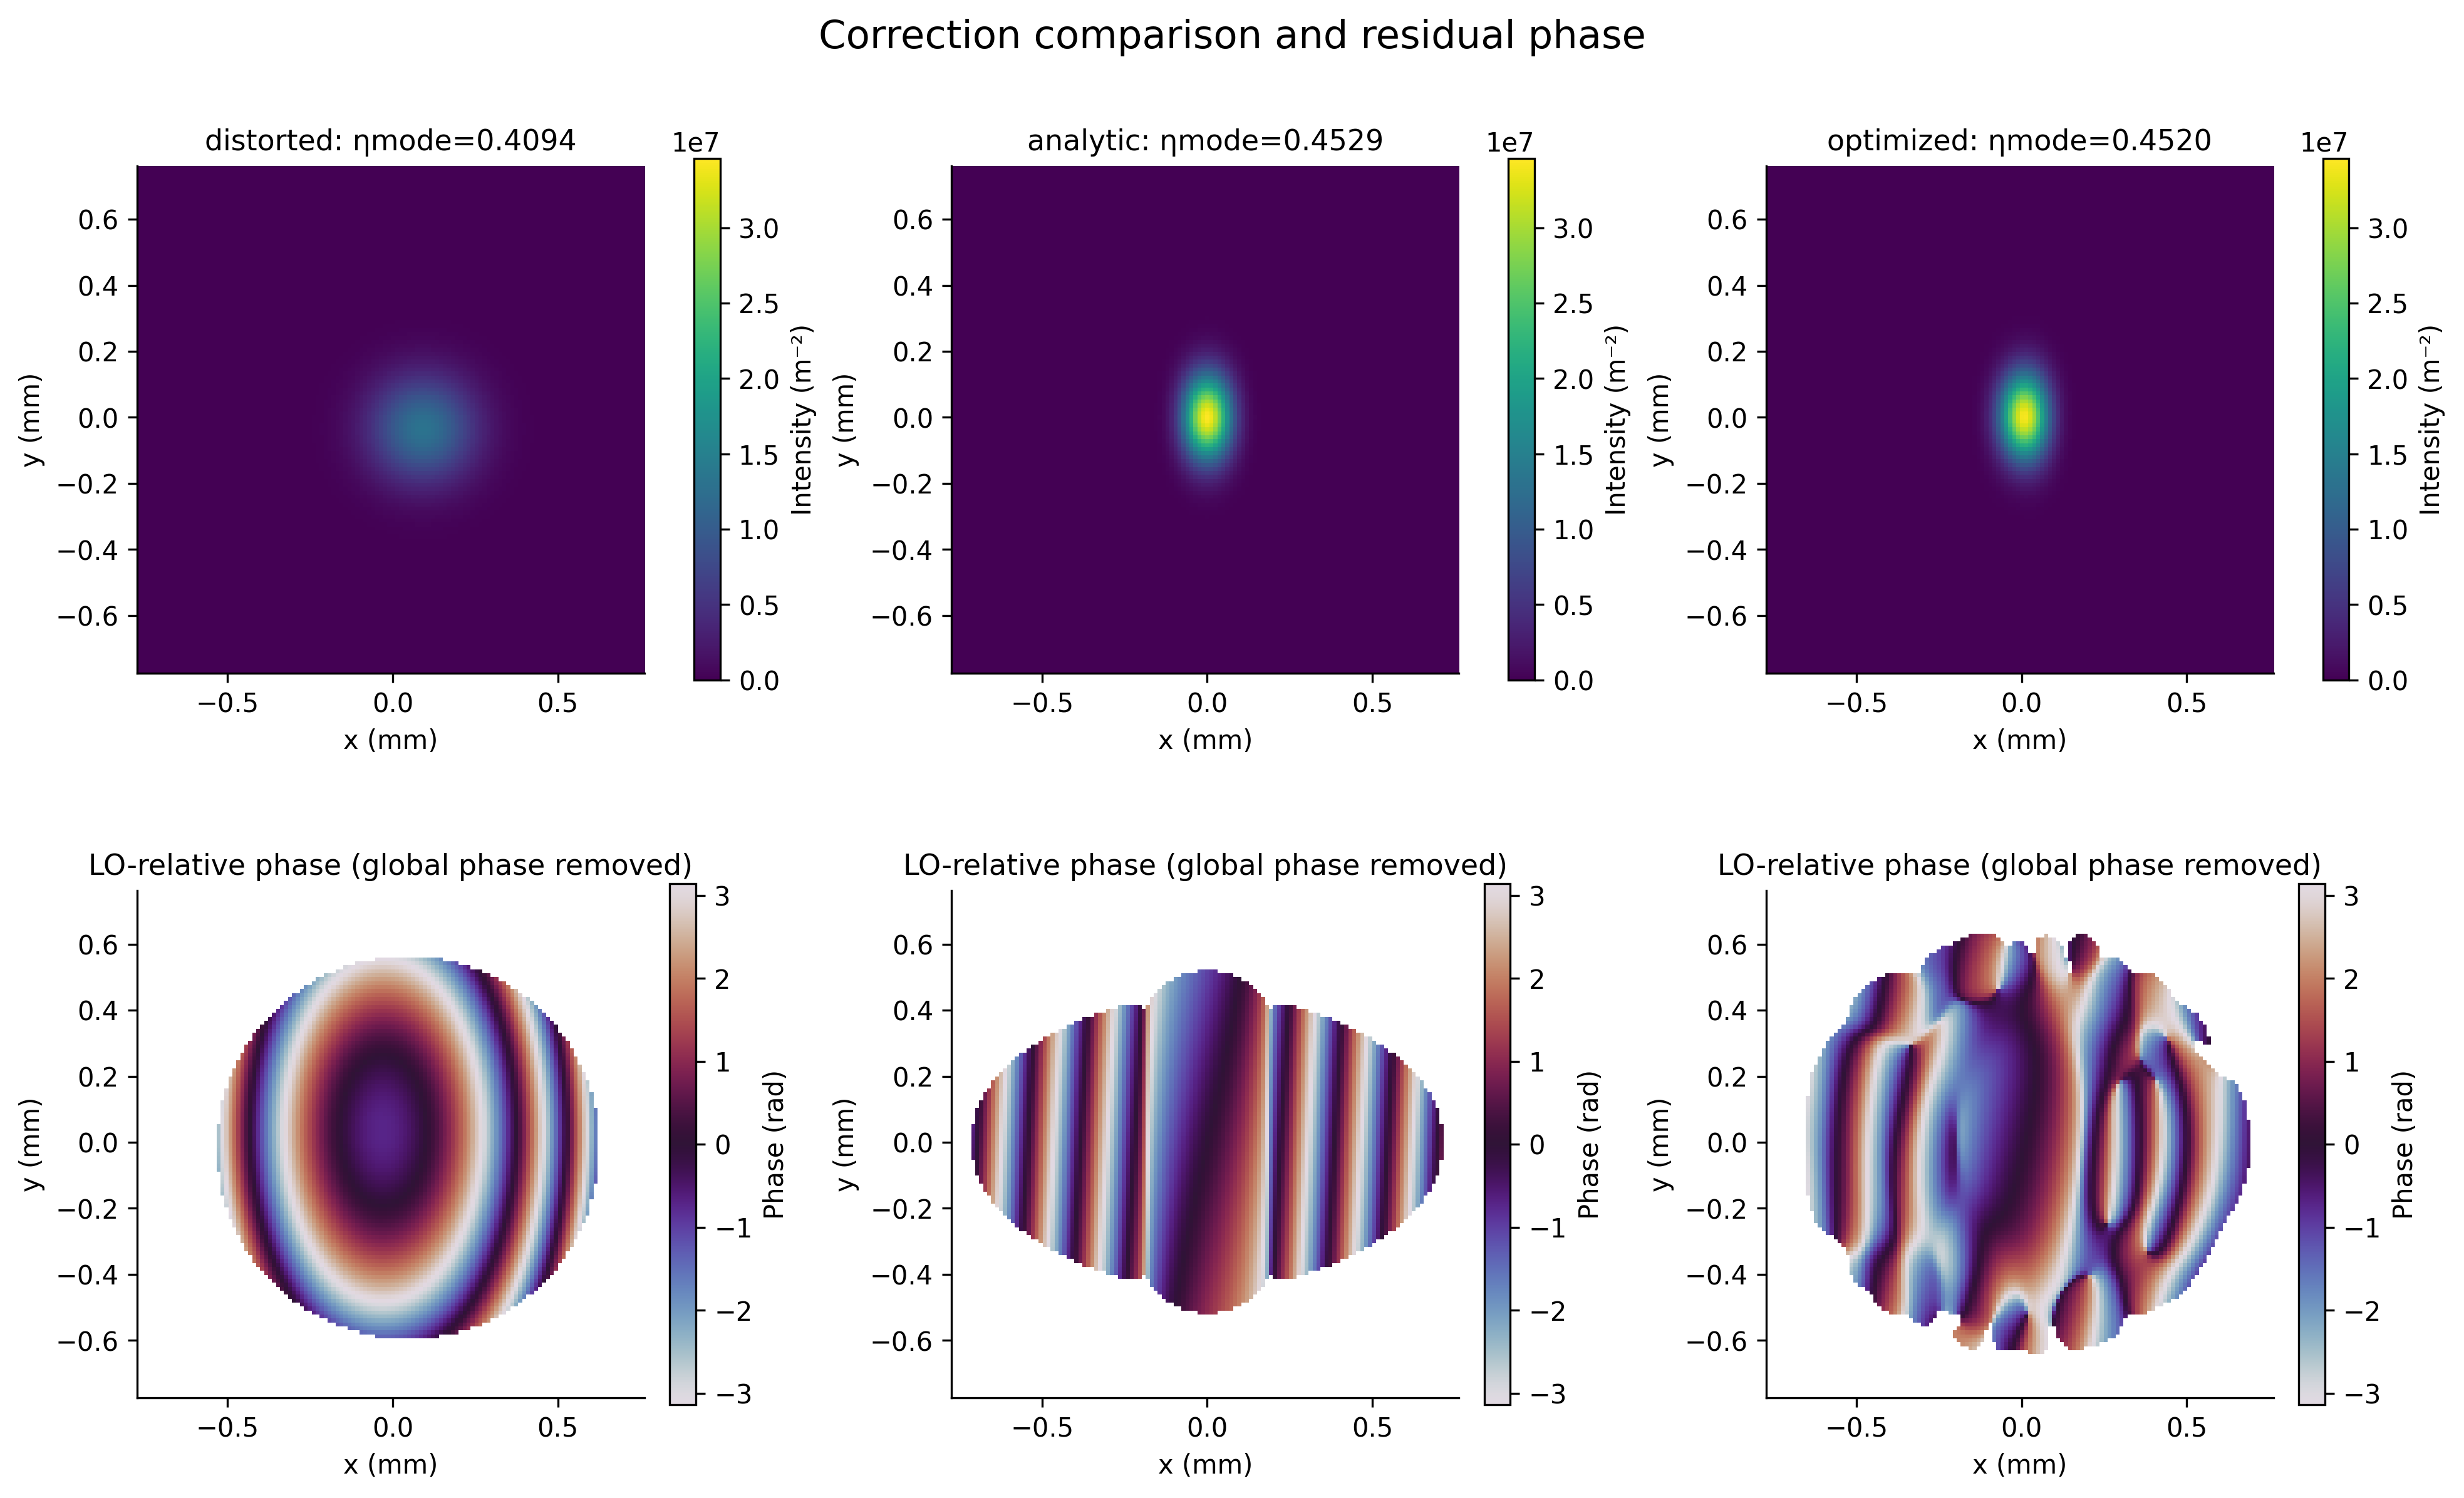
\includegraphics[width=0.98\textwidth]{../results/figures/03_comparison.png}
\caption{Representative detector fields for the three correction choices: distorted without correction, fixed analytic correction, and trained correction. The upper row shows intensity and the lower row shows LO-relative residual phase. Global overlap phase is removed only for residual-phase visualization, not from the stored optical metrics. These are representative fields, not distribution means; ideal and lossy reference values are reported in Table~\ref{tab:principal}.}
\label{fig:comparison}
\end{figure*}

\begin{table*}[!t]
\caption{Representative Optical and Homodyne Results (Theory Unless Marked Empirical)}
\label{tab:principal}
\centering\small
\begin{tabular}{lrrrrrr}
\toprule
Case & $\etam$ & $\Topt$ & $\etal$ & SNR (linear) & $\operatorname{Var}(Y)$ & Empirical $\operatorname{Var}(Y)$\\
\midrule
Ideal & 1.000000 & 1.000000 & 0.720000 & 2.796117 & 3.910000 & 3.928231\\
Distorted/no mask & 0.409409 & 1.000000 & 0.294774 & 1.144754 & 2.209097 & 2.211312\\
Fixed analytic & 0.452898 & 1.000000 & 0.326087 & 1.266356 & 2.334347 & 2.343929\\
Trained & 0.452023 & 1.000000 & 0.325457 & 1.263909 & 2.331827 & 2.333198\\
Lossy, trained mask & 0.201999 & 0.061736 & 0.008979 & 0.034869 & 1.065915 & 1.061700\\
\bottomrule
\end{tabular}
\end{table*}

Figure~\ref{fig:mask} displays the selected phase. Its wrapped range is $[-3.13482,3.12529]$ rad, but a broad phase histogram does not imply that every phase value is optically important: unilluminated and weakly illuminated pixels are included. Moreover, global phase is irrelevant to the overlap magnitude, and low-power regions can admit very different phase patterns with nearly identical scores. Mask appearance is therefore not, by itself, evidence of unique physical structure or manufacturability.

\begin{figure*}[!t]
\centering
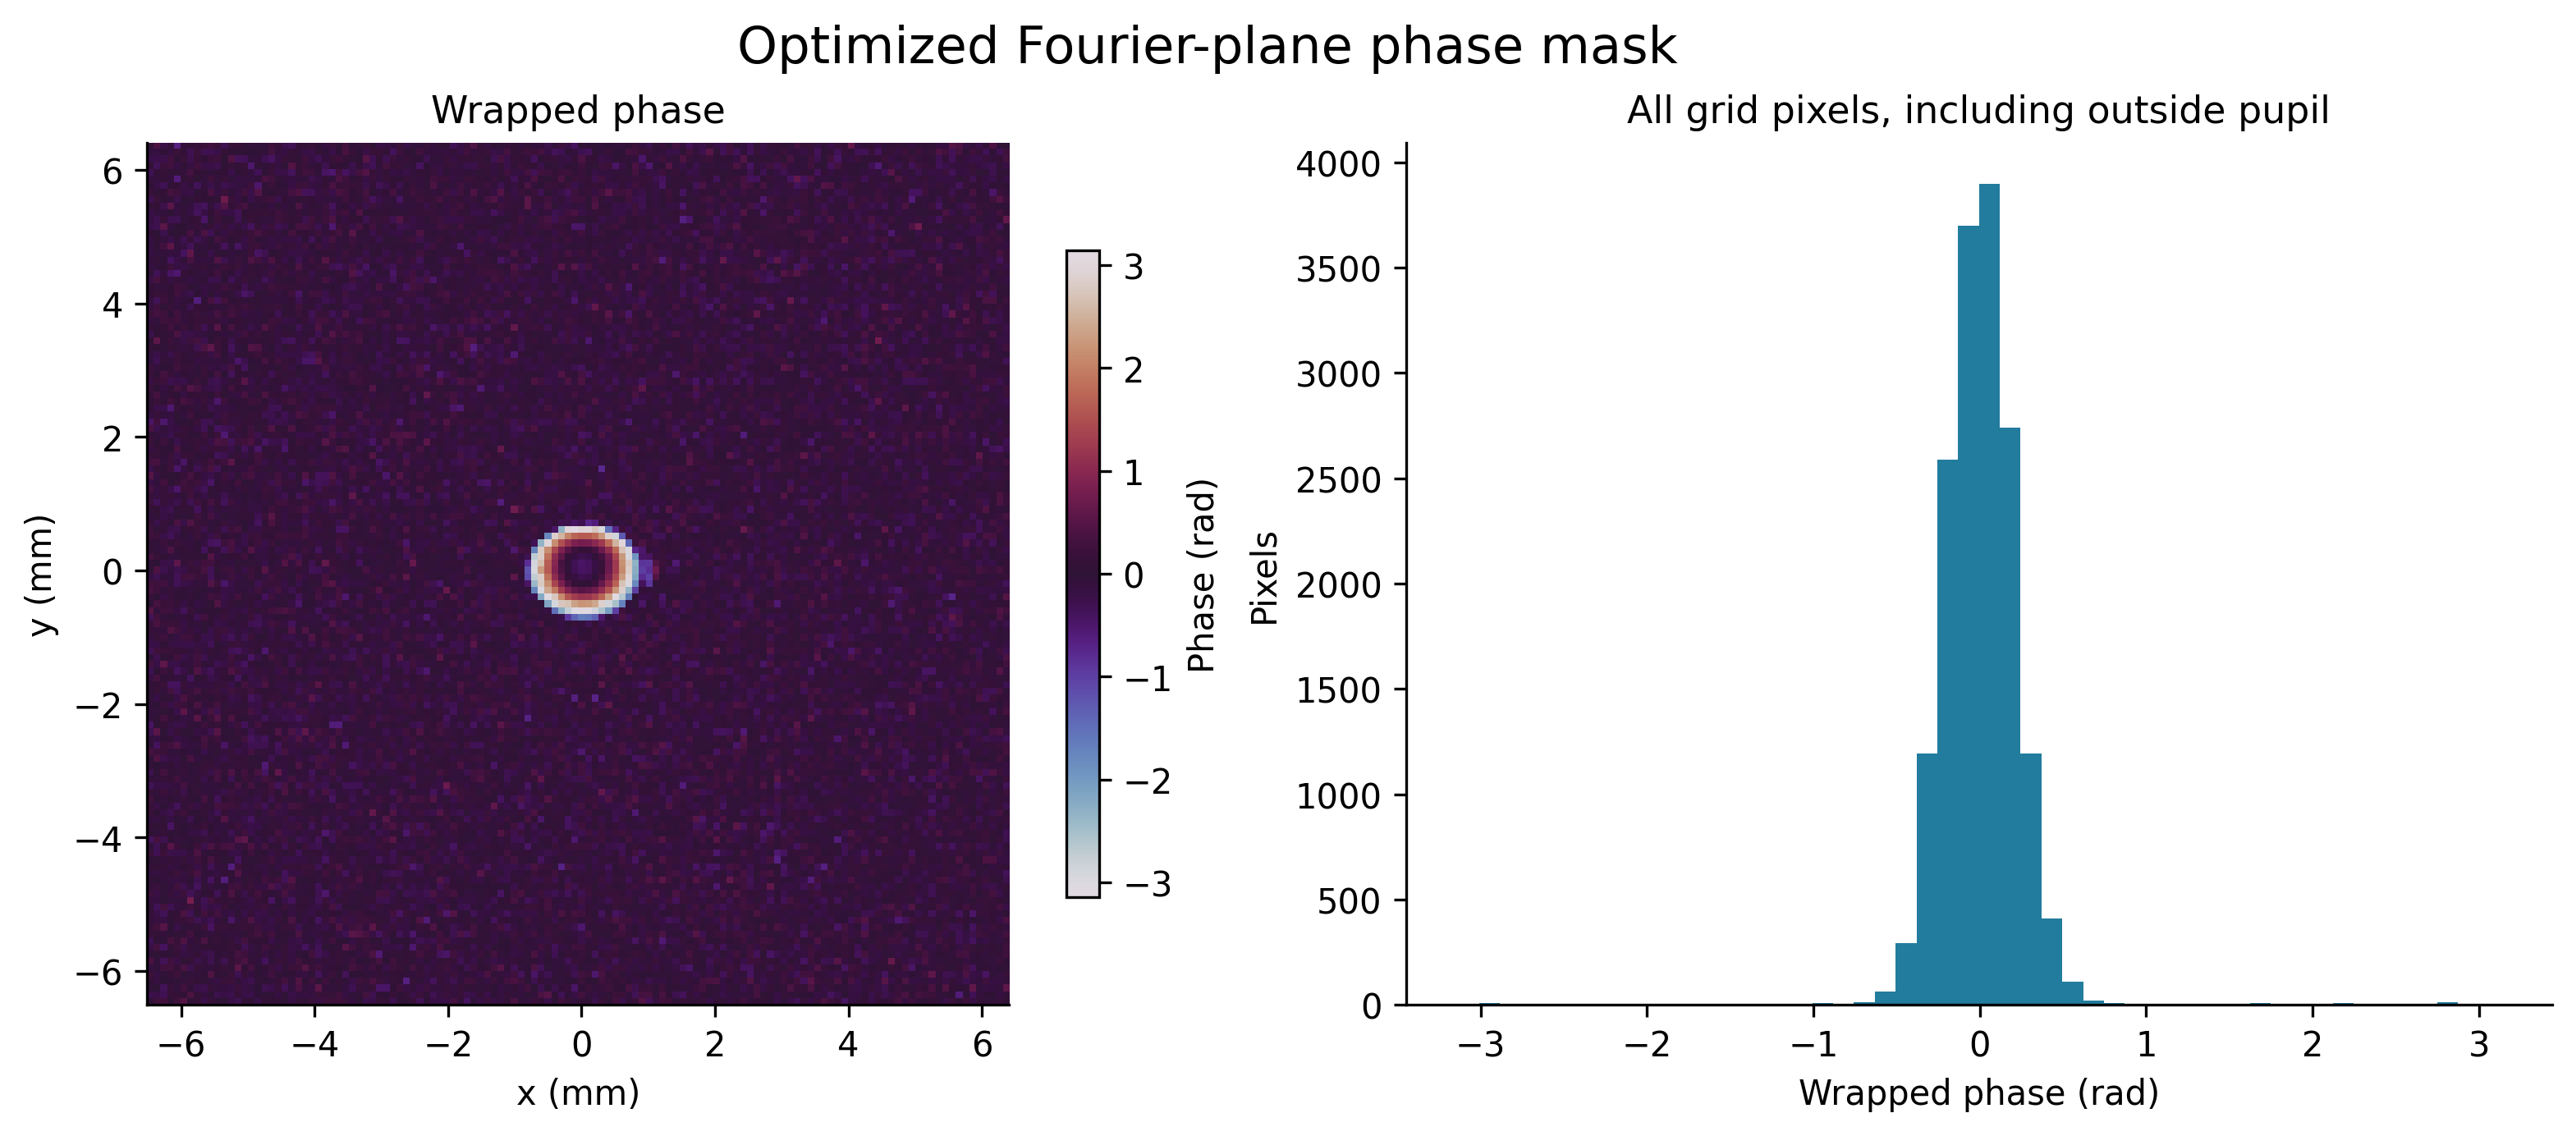
\includegraphics[width=0.9\textwidth]{../results/figures/04_mask.png}
\caption{Validation-selected Fourier-plane phase mask and pixel-phase distribution. The phase is continuous during optimization and wrapped for export/display. Fourier sampling pitch is $100.911~\mu$m. The histogram includes weakly illuminated or unilluminated pixels; no minimum feature size, finite phase-level constraint, or material phase-to-depth relation was imposed. The saved radians array is not a fabrication-ready design.}
\label{fig:mask}
\end{figure*}

\subsection{Validation and Independent Generalization}
The selected checkpoint is initialization 2, iteration 54, with validation overlap 0.455778. Figure~\ref{fig:learning} presents the archived learning histories. All runs use the same training and validation fields, so the initialization envelope is a range across optimization starts, not a confidence interval across independent physical datasets. Choosing the maximum validation score among many checkpoints may itself overfit a small validation set; the untouched test set is therefore essential.

\begin{figure*}[!t]
\centering
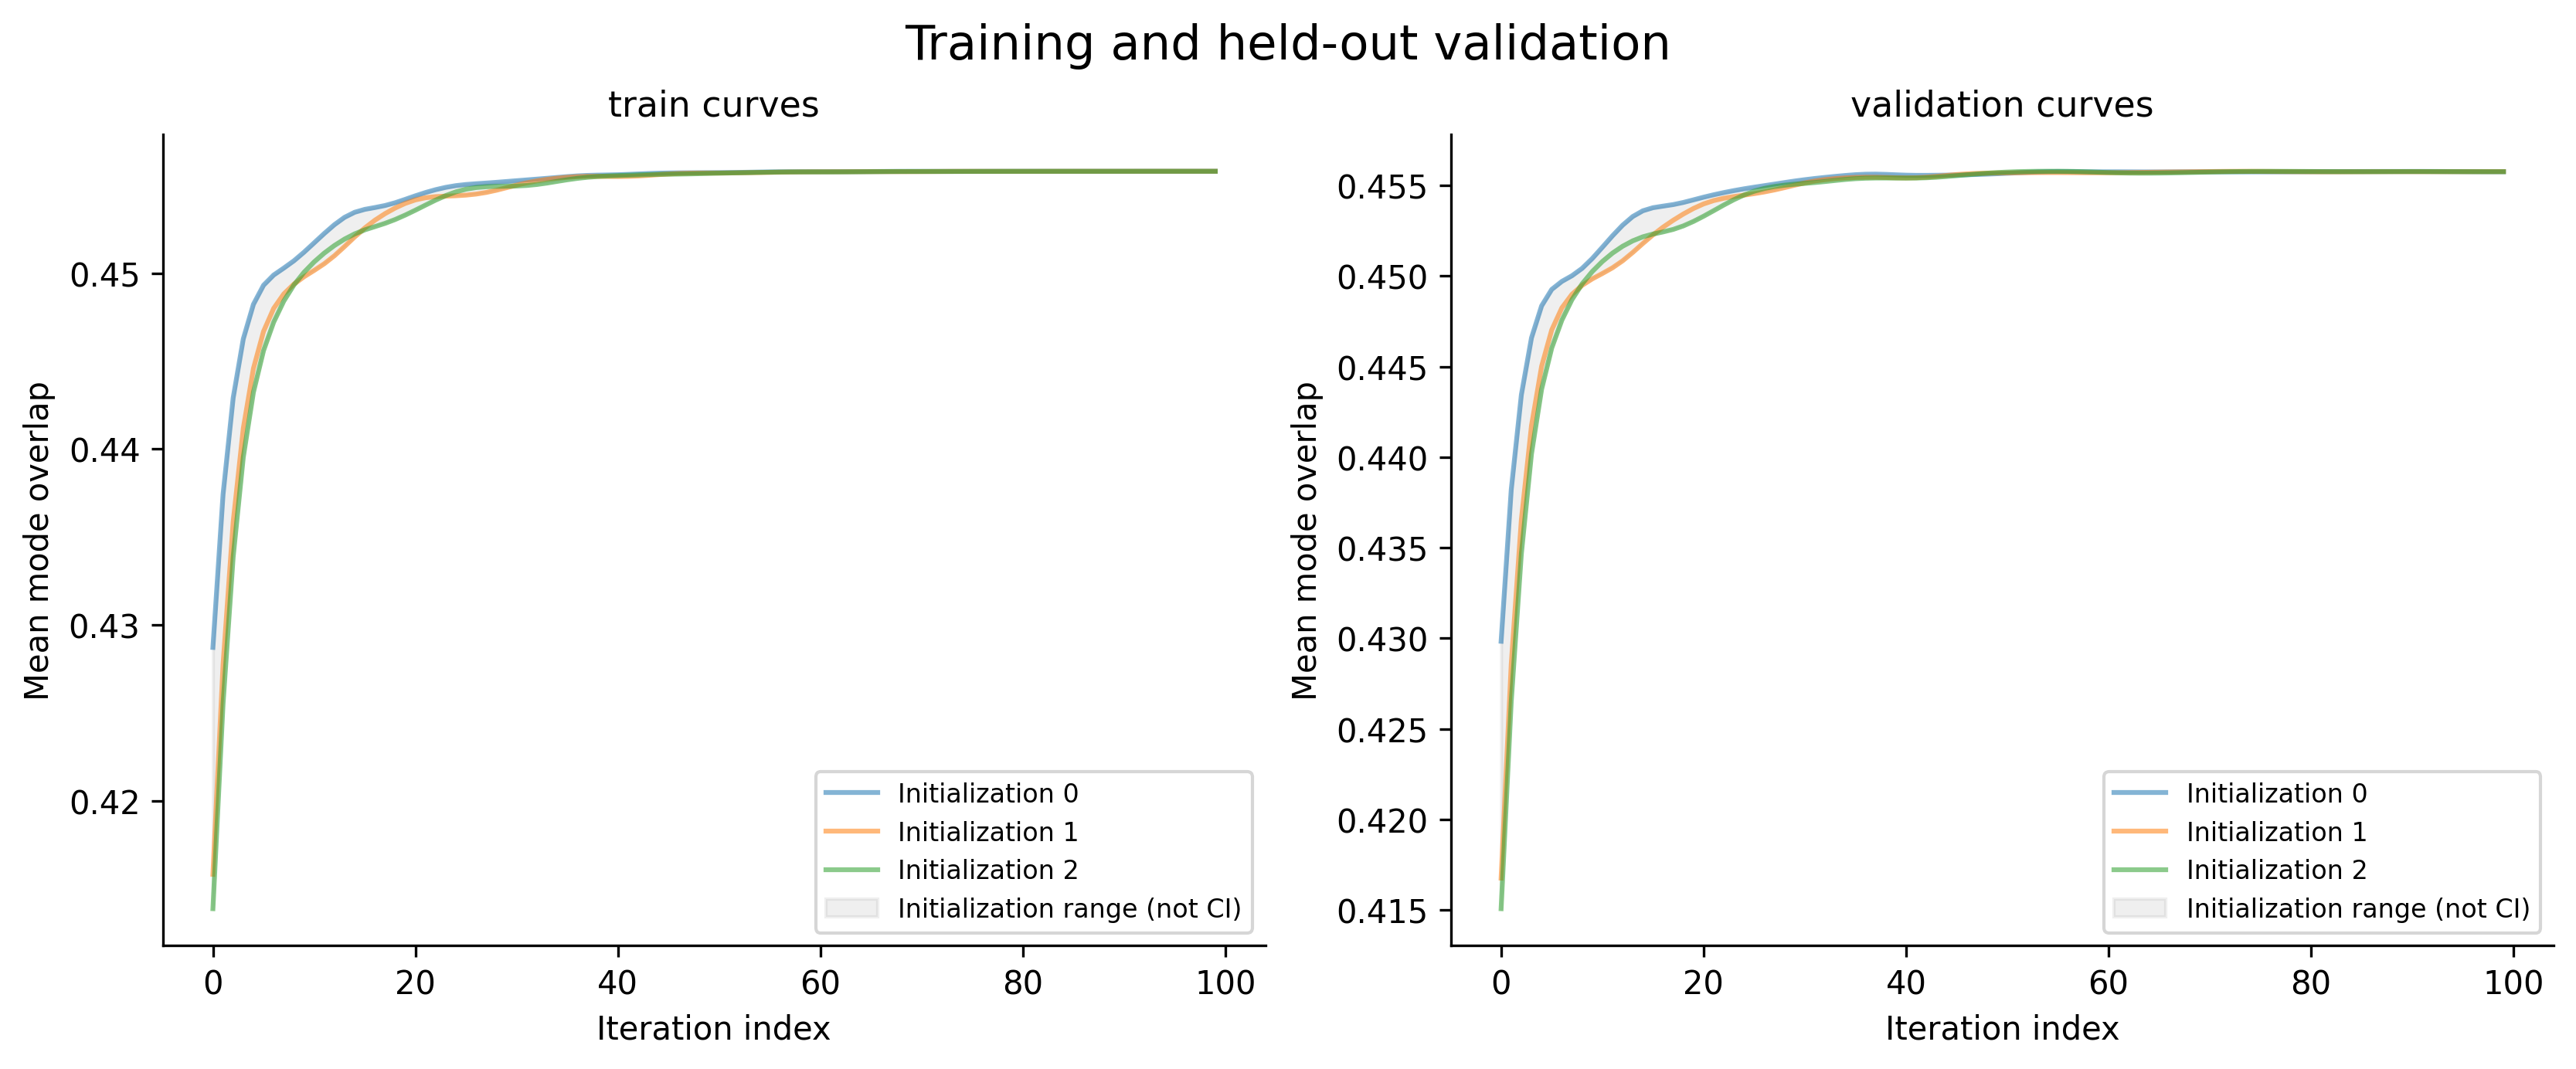
\includegraphics[width=0.94\textwidth]{../results/figures/05_learning.png}
\caption{Training and held-out validation histories over three initializations. Adam updates use training fields only; post-update validation selects the retained checkpoint across all runs. The selected zero-based initialization and iteration are 2 and 54, respectively, with validation overlap 0.455778. Initialization ranges are not statistical confidence bands. The separate test split is not used to choose these histories or the mask.}
\label{fig:learning}
\end{figure*}

Table~\ref{tab:paired} gives the independent distribution statistics and all three archived paired comparisons. The trained-minus-uncorrected difference is positive throughout its 95\% interval. Analytic-minus-uncorrected correction also has a positive interval. In contrast, the trained-minus-analytic mean is only 0.000268, with interval $[-0.001372,0.001907]$. The available evidence supports phase correction for this distribution, but cannot establish that the trained mask is better than the fixed analytic comparator.

The near equality is scientifically useful rather than an optimization failure that should be hidden. A representative analytic phase mask is a strong baseline for a relatively concentrated distribution of smooth distortions. A learned phase mask has more freedom, but freedom alone is not a measured benefit. Demonstrating a robust advantage would require different evidence, such as larger independent seed sweeps or a justified distribution where a single representative analytic phase is inadequate; those experiments are outside this archived study.

\begin{table*}[!t]
\caption{Independent Test Distribution and Paired Comparisons ($n=24$, Seed 303)}
\label{tab:paired}
\centering\small
\begin{tabular}{lrrrl}
\toprule
Correction & Mean overlap & Standard deviation & Standard error & Mean throughput\\
\midrule
No mask & 0.431225 & 0.070354 & 0.014361 & $\simeq1$\\
Fixed analytic & 0.469958 & 0.070466 & 0.014384 & $\simeq1$\\
Trained & 0.470226 & 0.072116 & 0.014721 & $\simeq1$\\
\midrule
Paired difference & Mean difference & Standard error & \multicolumn{1}{c}{95\% interval} & Interpretation\\
\midrule
Trained $-$ no mask & 0.039001 & 0.001546 & [0.035802, 0.042199] & Positive improvement supported\\
Trained $-$ analytic & 0.000268 & 0.000792 & [$-0.001372$, 0.001907] & Superiority not demonstrated\\
Analytic $-$ no mask & 0.038733 & 0.002020 & [0.034555, 0.042911] & Positive improvement supported\\
\bottomrule
\end{tabular}
\end{table*}

\subsection{Tolerance Scan and Irrecoverable Amplitude Damage}
The deterministic heatmaps in Fig.~\ref{fig:robustness} show substantial variation over displacement and defocus. The no-mask overlap ranges from 0.04247 to 0.80529, the analytic mask from 0.04559 to 0.80731, and the trained mask from 0.04538 to 0.82041. These extrema occur over a prescribed finite grid, not over a probability distribution. They neither establish uniform improvement nor supply a manufacturing tolerance certificate.

\begin{figure*}[!t]
\centering
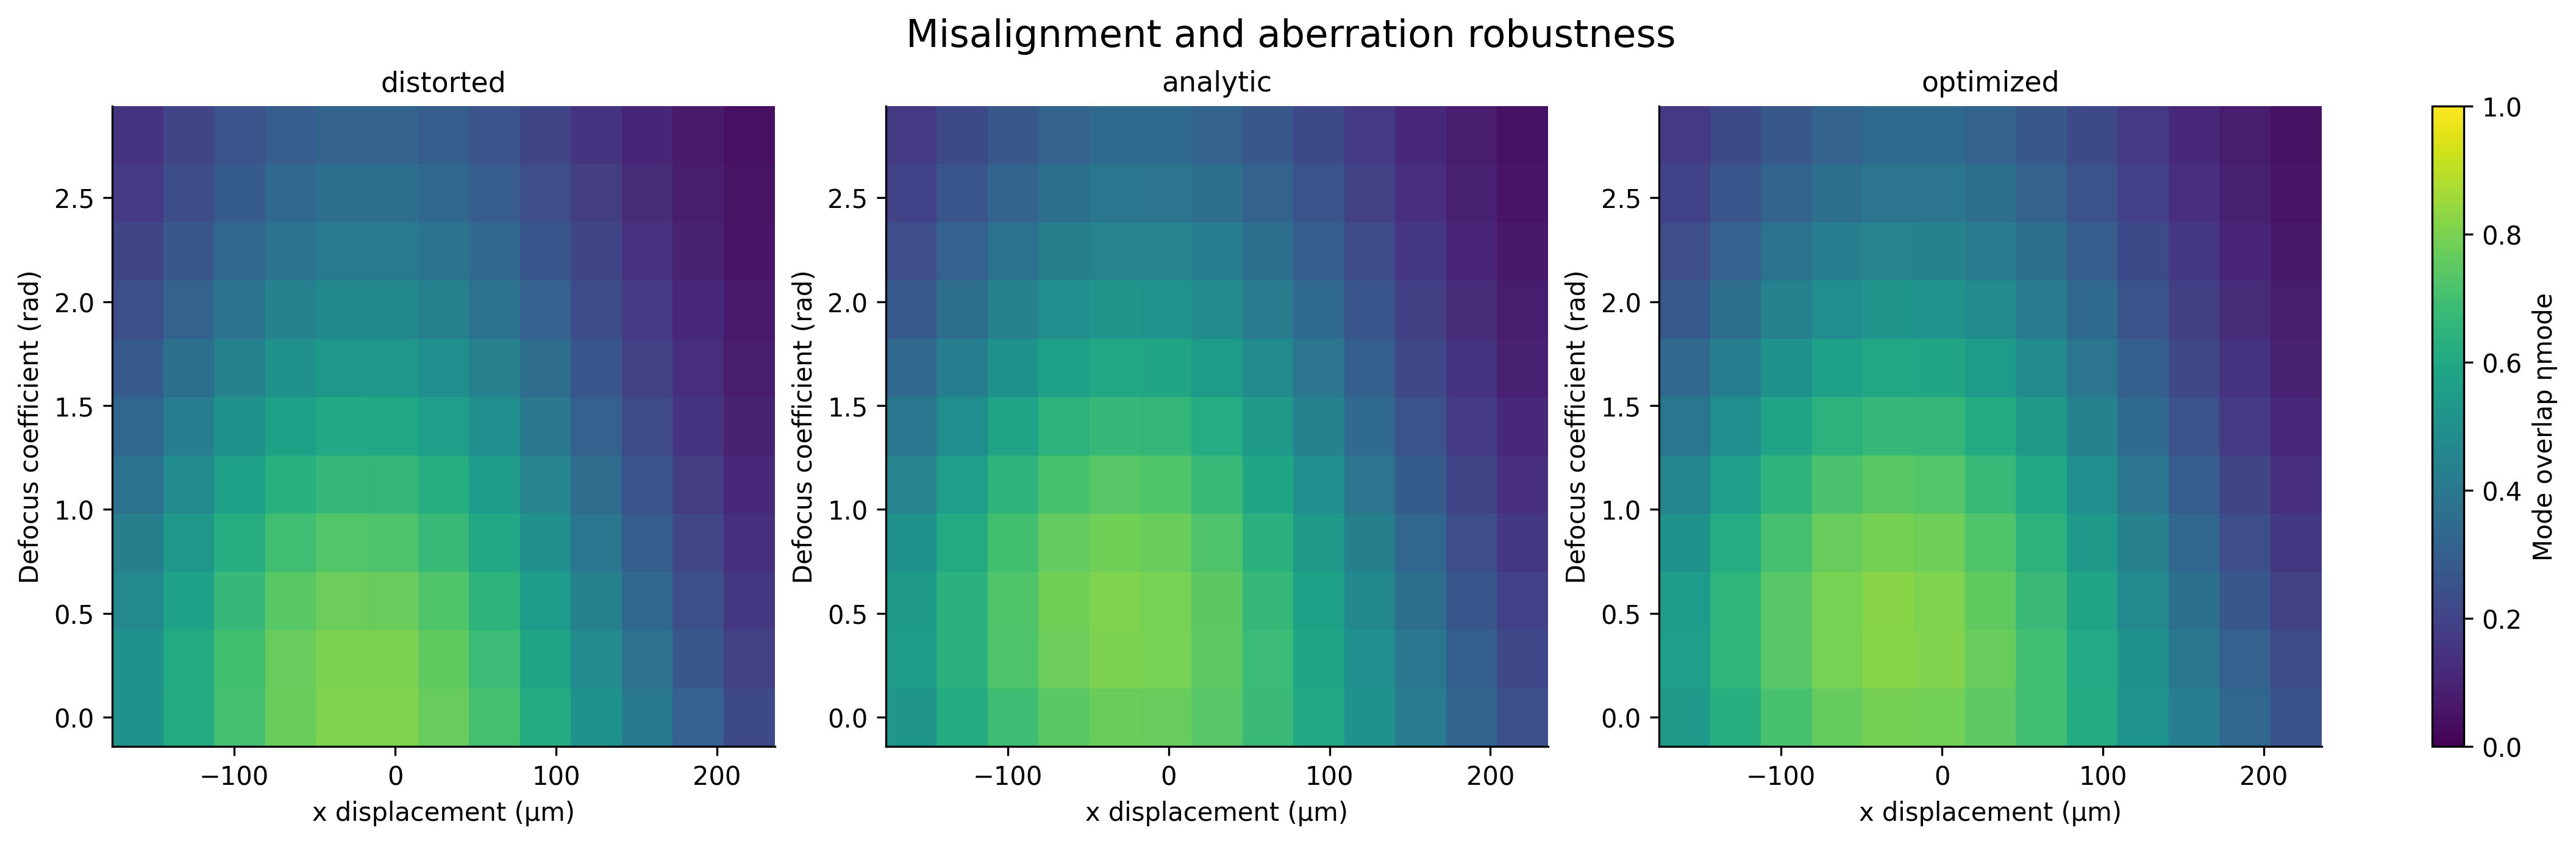
\includegraphics[width=0.98\textwidth]{../results/figures/06_robustness.png}
\caption{Unretrained displacement--defocus sensitivity scan for no correction, fixed analytic correction, and trained correction. Horizontal displacement is swept from $-160$ to $220~\mu$m and defocus coefficient from 0 to 2.8 rad; the other distortion parameters remain at their means. The finite deterministic grid illustrates sensitivity outside one representative field, but is not a statistical confidence map or a complete alignment budget.}
\label{fig:robustness}
\end{figure*}

For a stronger negative control, the representative source is multiplied by $\mathbf{1}_{x>0}\sqrt{0.08}$ before the relay. Its pre-relay power is 0.0622056774 and post-pupil power is 0.0617361971 relative to the original unity input. Because the displaced source lies asymmetrically across the half-plane boundary, the transmitted power is not simply one-half of 0.08. The archived trained mask gives normalized overlap 0.201999, but low performance of one reused mask alone would not demonstrate impossibility of correction.

Equation~\eqref{eq:bound} supplies the stronger conclusion. For this actual damaged field and pupil, the attainable phase-only overlap ceiling is 0.2438595833 and the coupled-power ceiling is 0.0150549633. The first is strictly below unity because of spectral-magnitude mismatch; the second also accounts for irreversible loss. Thus even ideal phase alignment cannot restore the original useful signal. The independent acceptance test explicitly constructs a lossy field, applies analytic phase alignment, and verifies attainment of the computed bound and the hierarchy of powers. That test validates the bound implementation; it does not convert the sampled ceiling into an experimentally measured limit.

\section{Quantum-Noise Interface and Independent Validation}
\subsection{Passive Loss in Shot-Noise Units}
Before translating overlap into communication performance, it is necessary to establish the quantum-noise convention. We use $\hat X=\hat a+\hat a^\dagger$ and $\hat P=(\hat a-\hat a^\dagger)/i$, corresponding to $\hbar=2$ and vacuum covariance $I$. A passive pure-loss channel transforms Gaussian mean vector $\boldsymbol m$ and covariance $V$ according to \cite{weedbrook,sfloss}
\begin{equation}
 \boldsymbol m_{\rm out}=\sqrt{T}\boldsymbol m_{\rm in},\qquad
 V_{\rm out}=TV_{\rm in}+(1-T)I.
 \label{eq:quantum}
\end{equation}
For a coherent state, $V_{\rm in}=I$, so $V_{\rm out}=I$ at every transmission, including complete loss. Vacuum fluctuations are not multiplied down with the coherent signal. Likewise, cascading independent passive efficiency factors does not require adding a new full shot-noise unit for every factor; their composite coherent-state output retains one unit of vacuum variance.

Mode mismatch can be represented as effective loss for the selected coherent mode when the unobserved orthogonal modes are vacuum and the receiver is otherwise ideal. This is the modeling assumption connecting Eq.~\eqref{eq:eta} to Eq.~\eqref{eq:quantum}. The study does not propagate arbitrary non-Gaussian multimode states or derive security against an adversarial channel.

\subsection{Executed Gaussian Backend Versus Monte Carlo Sampling}
An isolated Strawberry Fields 0.23.0 Gaussian backend \cite{sfdocs} executes one-mode vacuum and coherent preparations followed by \texttt{LossChannel}. Eleven transmissivities from zero to unity are used for each input, yielding 22 checked states. The coherent amplitude is $\alpha=1-0.4i$, hence the input mean is $(2,-0.8)$ and covariance is $I$. Both output quadrature means and the full covariance are compared with Eq.~\eqref{eq:quantum}. The archived maximum absolute backend mean error is $2.22\times10^{-16}$ and maximum covariance error is zero.

Figure~\ref{fig:quantum} is deliberately presented before receiver performance. Its empirical points are independent NumPy multivariate-normal samples, not Strawberry Fields measurement trajectories. With 100,000 samples at each transmission, the maximum sampled mean and variance deviations are 0.00656945 and 0.00776008, respectively. These Monte Carlo deviations must not be confused with the near-machine-precision backend moment errors. The figure has no per-point uncertainty bars and no separately sampled vacuum curve; the vacuum state is checked by the backend and by automated tests.

\begin{figure*}[!t]
\centering
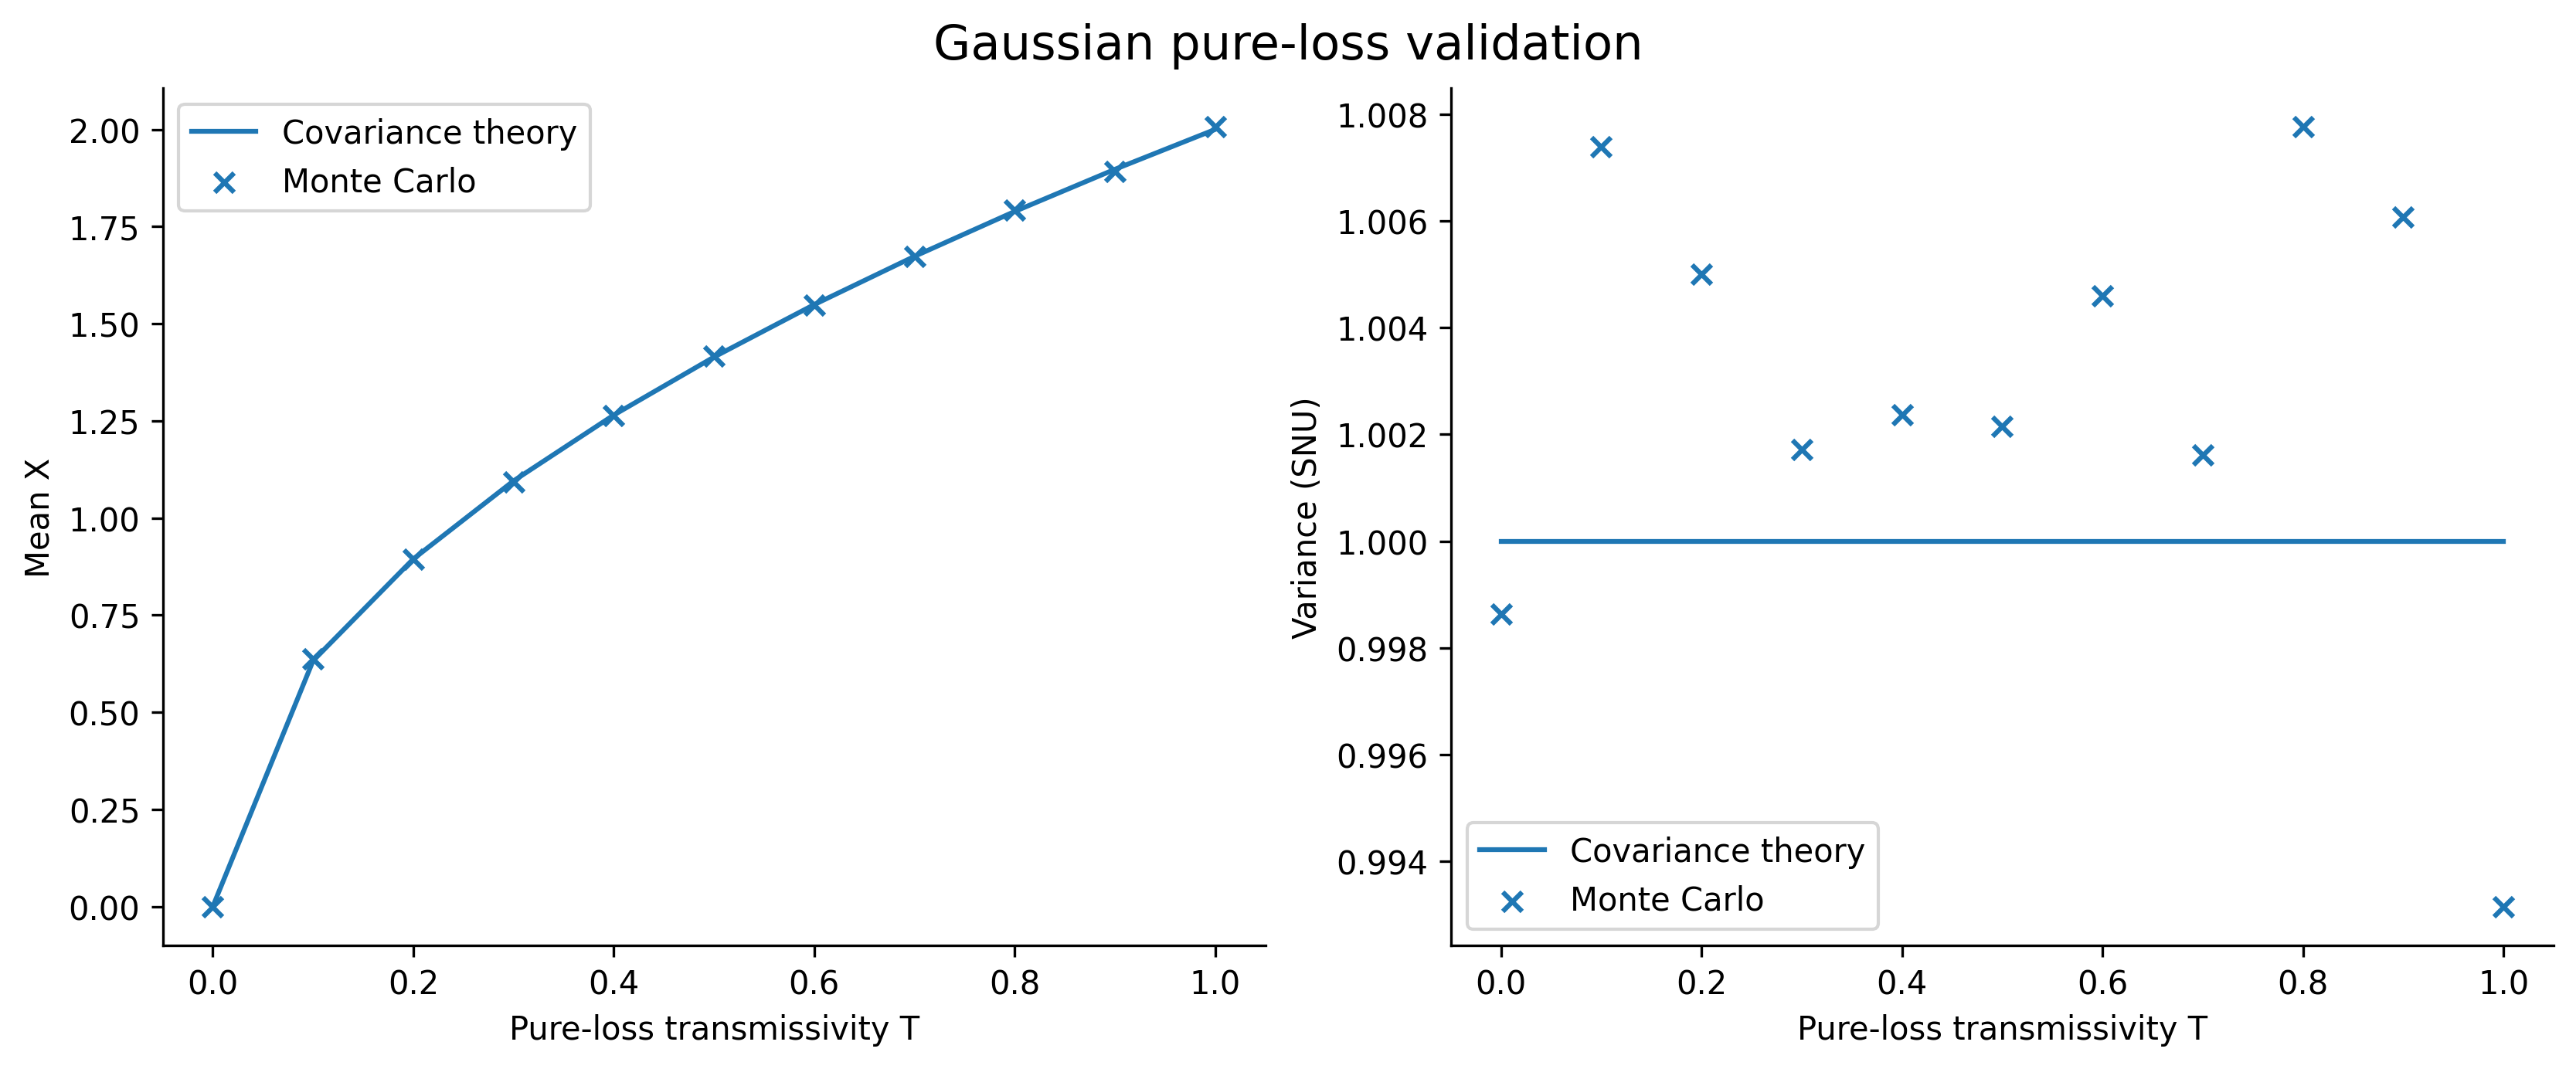
\includegraphics[width=0.94\textwidth]{../results/figures/10_quantum.png}
\caption{Pure-loss quantum-limit cross-check, placed here as Fig.~7 although the archived asset is named \texttt{10\_quantum.png}. Coherent input mean $(2,-0.8)$ scales as $\sqrt{T}$ while covariance remains the identity in shot-noise units. Plotted empirical values are NumPy Monte Carlo summaries, with 100,000 samples at each transmission; Strawberry Fields separately verifies vacuum and coherent Gaussian moments for 22 cases. Small variance departures from unity are finite-sample fluctuations, not squeezing. This figure does not include excess or electronic noise.}
\label{fig:quantum}
\end{figure*}

The isolation boundary is also tested. If the backend interpreter is unavailable, times out, or exits unsuccessfully, the software records the error and labels an exact covariance-matrix fallback. Conversely, a backend that returns physically inconsistent moments fails validation rather than silently falling back. The committed evidence identifies actual Strawberry Fields execution, not fallback. Backend execution is an independent software consistency check against the Gaussian model, not experimental quantum validation.

\section{Homodyne Statistics and Receiver Performance}
\subsection{One-Quadrature Observation Model}
Alice prepares independent zero-mean Gaussian variables $X_A,P_A$ with variance $V_A$. For residual LO angle $\theta$, define the matched variable
\begin{equation}
 X_\theta=X_A\cos\theta-P_A\sin\theta.
\end{equation}
The one-quadrature observation is
\begin{equation}
 Y=\sqrt{\etal}X_\theta+Z_0+Z_{\rm rec}+Z_{\rm el},
 \label{eq:homodyne}
\end{equation}
where the independent noise terms have variances $1$, $\xi_{\rm rec}$, and $v_{\rm el}$. Excess and electronic noise are receiver-referred additive variances, not input-referred security parameters. Baseline phase compensation sets $\theta=0$ using the simulated overlap phase. Perfect phase knowledge is an assumption, not an estimated receiver capability.

Six spawned random streams separately produce $X_A$, $P_A$, vacuum noise, receiver noise, electronics noise, and independent vacuum calibration. The expected variance and matched-variable SNR are
\begin{align}
 \operatorname{Var}(Y)&=\etal V_A+1+\xi_{\rm rec}+v_{\rm el},\label{eq:variance}\\
 \mathrm{SNR}&=\frac{\etal V_A}{1+\xi_{\rm rec}+v_{\rm el}}.
 \label{eq:snr}
\end{align}
For uncompensated phase, the SNR relative to the original $X_A$, rather than $X_\theta$, is instead
\begin{equation}
 \mathrm{SNR}_{X_A}=
 \frac{\etal V_A\cos^2\theta}
 {1+\xi_{\rm rec}+v_{\rm el}+\etal V_A\sin^2\theta}.
 \label{eq:phasenoise}
\end{equation}
This distinction is important even though the archived baseline is phase compensated: isotropic modulation makes total variance insensitive to $\theta$, while correlation with Alice's original variable can vanish.

\subsection{Conditioning, Calibration, and Variance}
Figure~\ref{fig:homodyne} distinguishes residual noise, finite-bin conditioned observations, and Alice--Bob scatter. Residuals are the known latent sum of the three noise contributions. They are not reconstructed residuals from a receiver estimator. Conditional observations select $|X_A|\leq0.1\sqrt{V_A}$, or $|X_A|\leq0.2$ for this baseline; finite bin width leaves a small signal contribution. They are therefore not exactly delta-conditioned coherent states.

\begin{figure*}[!t]
\centering
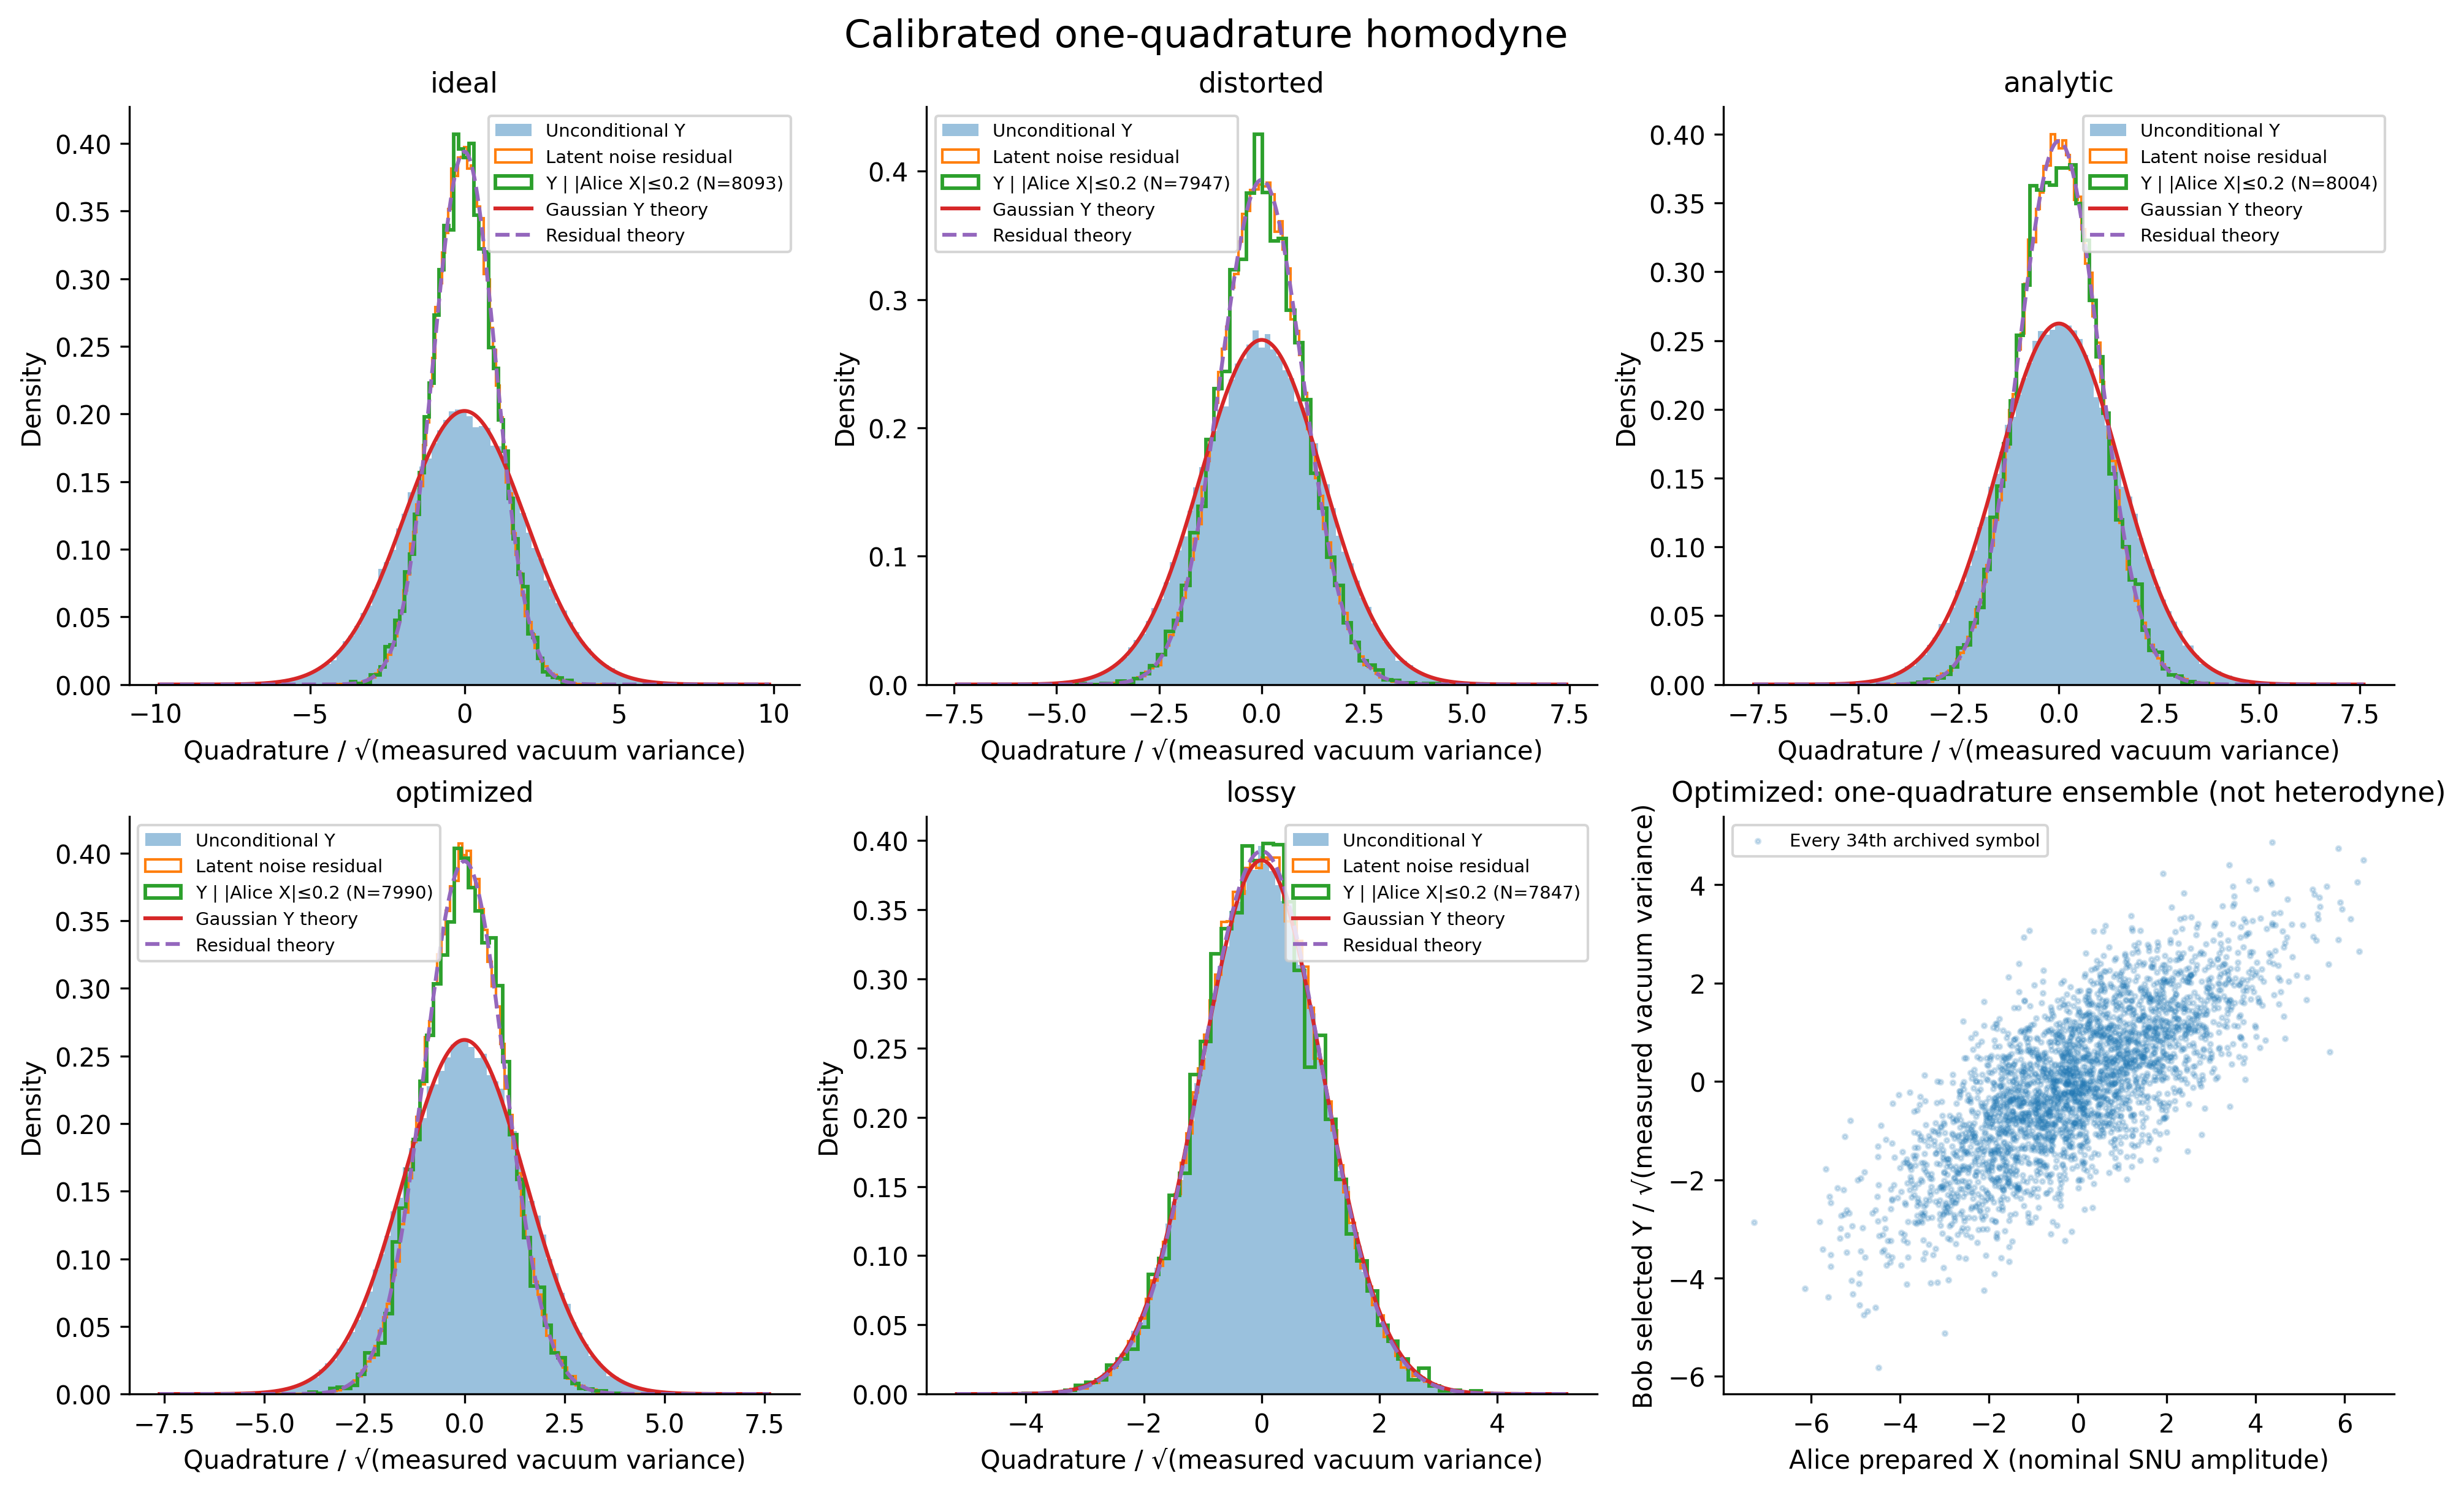
\includegraphics[width=0.98\textwidth]{../results/figures/07_homodyne.png}
\caption{One-quadrature homodyne ensembles with independent vacuum calibration: residual-noise histograms, finite Alice-bin conditional distributions, and Alice-$X$/Bob-$Y$ scatter. Each principal case contains 100,000 simulated symbols. Residuals use known sampler components; conditional samples are actual observations selected in $|X_A|\leq0.2$, not residuals relabeled as conditional data. Scatter pairs Alice's prepared variable with one measured Bob quadrature across symbols and does not depict simultaneous $X/P$ or heterodyne detection. Plot calibration divides quadrature by the independent measured vacuum standard deviation.}
\label{fig:homodyne}
\end{figure*}

The archive stores conditional samples selected on $X_\theta$, whereas the plotting code selects original $X_A$. These selections coincide with the baseline phase compensation, but would differ off baseline. The stored scatter includes prepared $X_A$, $P_A$, their rotated combination, and measured $Y$ for 5000 symbols; storing both preparation variables is not a simultaneous quantum measurement by Bob.

The independent calibration variances for ideal, distorted, analytic, trained, and lossy cases are 1.004746, 1.001340, 1.010016, 1.005080, and 0.996482. The histogram display uses these calibration estimates, while Fig.~\ref{fig:variance} and Table~\ref{tab:principal} use nominal shot-noise units for variance comparisons. These conventions should not be mixed when assessing agreement.

\begin{figure*}[!t]
\centering
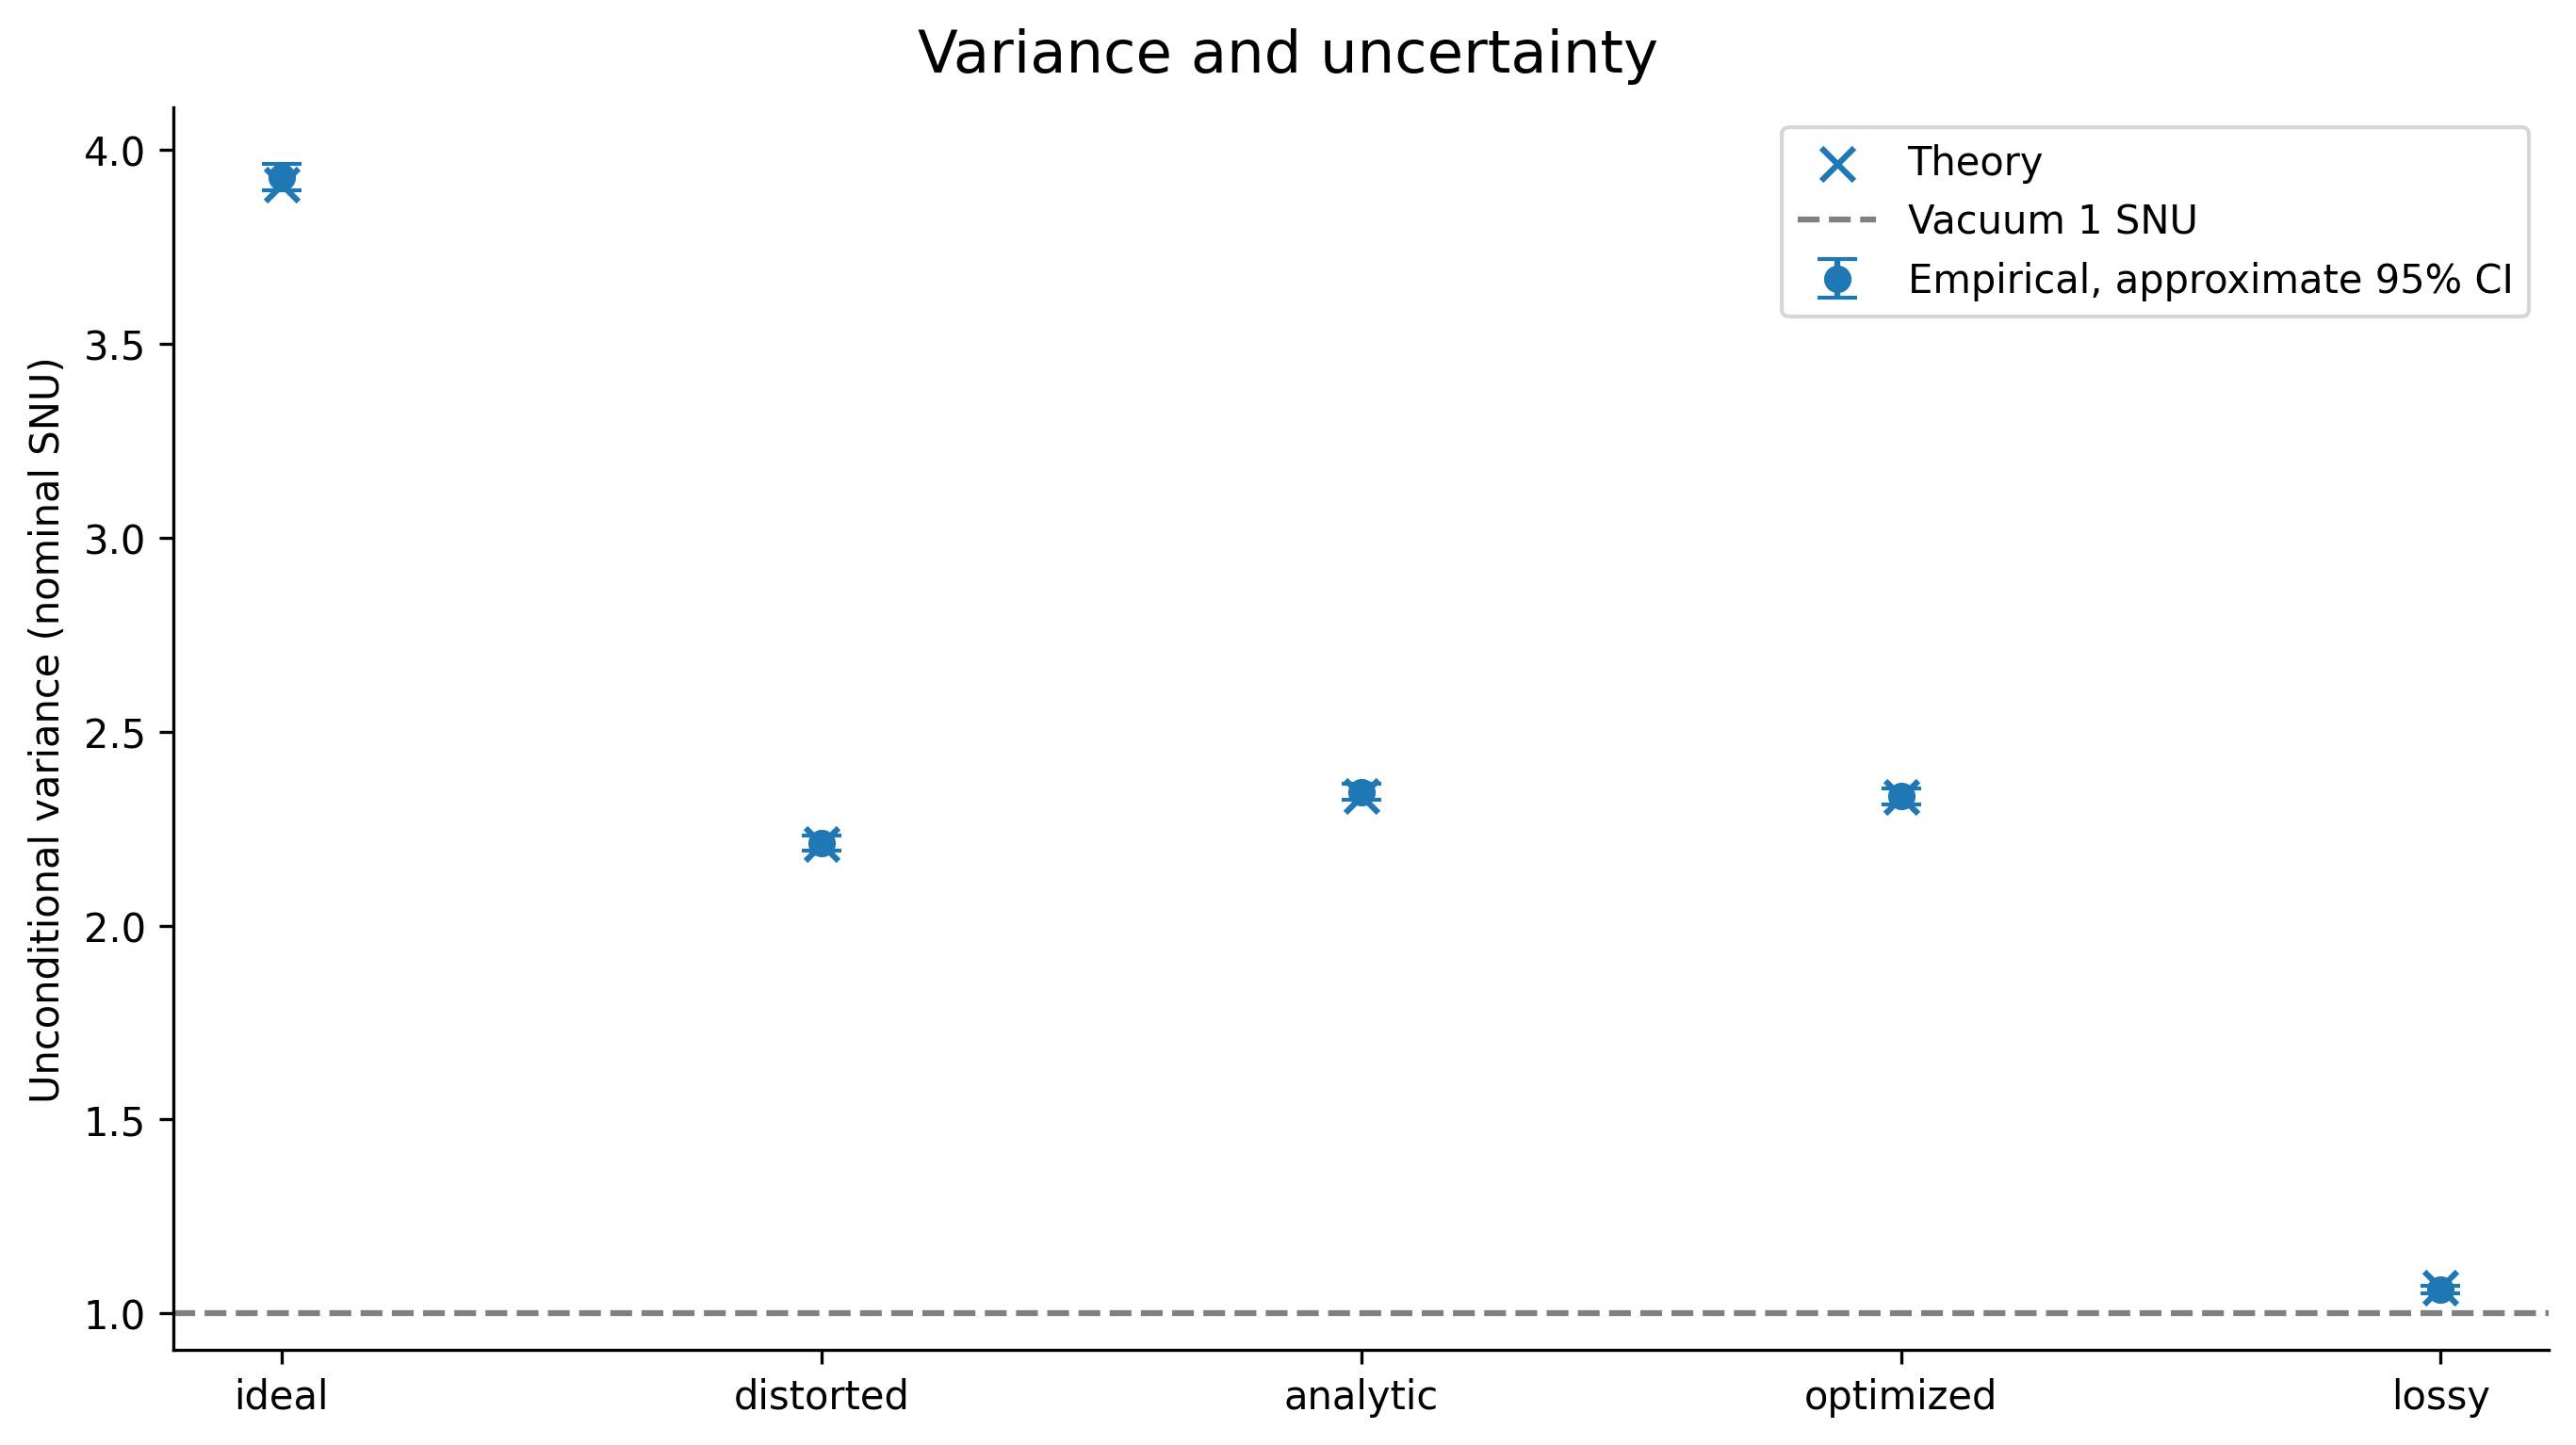
\includegraphics[width=0.94\textwidth]{../results/figures/08_variance.png}
\caption{Empirical and theoretical quadrature variances in nominal shot-noise units. Approximate 95\% intervals use the large-sample Gaussian sample-variance formula and contain the corresponding theory value in all five principal cases. They omit vacuum-calibration uncertainty and multiplicity corrections. Reduced unconditional variance after loss reflects diminished modulation, not sub-vacuum conditional noise or squeezing.}
\label{fig:variance}
\end{figure*}

For $n$ independent Gaussian samples, the displayed interval uses
\begin{equation}
 s_Y^2\ \pm\ 1.96s_Y^2\sqrt{\frac{2}{n-1}},
 \label{eq:varianceci}
\end{equation}
with a nonnegative lower endpoint. This is a large-sample approximation, not the exact chi-square interval. All five theoretical variances fall inside their archived intervals. For example, the trained case has empirical variance 2.333198, theory 2.331827, and interval [2.312747, 2.353650]. Separate acceptance tests use exact chi-square residual-variance intervals for pure-loss cases; those tests do not mean every plotted interval includes calibration uncertainty.

\subsection{SNR, Efficiency, and Interpretation}
Figure~\ref{fig:snr} shows theoretical SNR and the efficiency budget. The representative trained mask increases SNR relative to no correction, from 1.144754 to 1.263909, but the analytic case is slightly higher at 1.266356. This ordering follows the optical overlaps because the other factors and noise variances are fixed. It agrees with, rather than overrides, the lack of demonstrated trained superiority in the held-out comparison.

\begin{figure*}[!t]
\centering
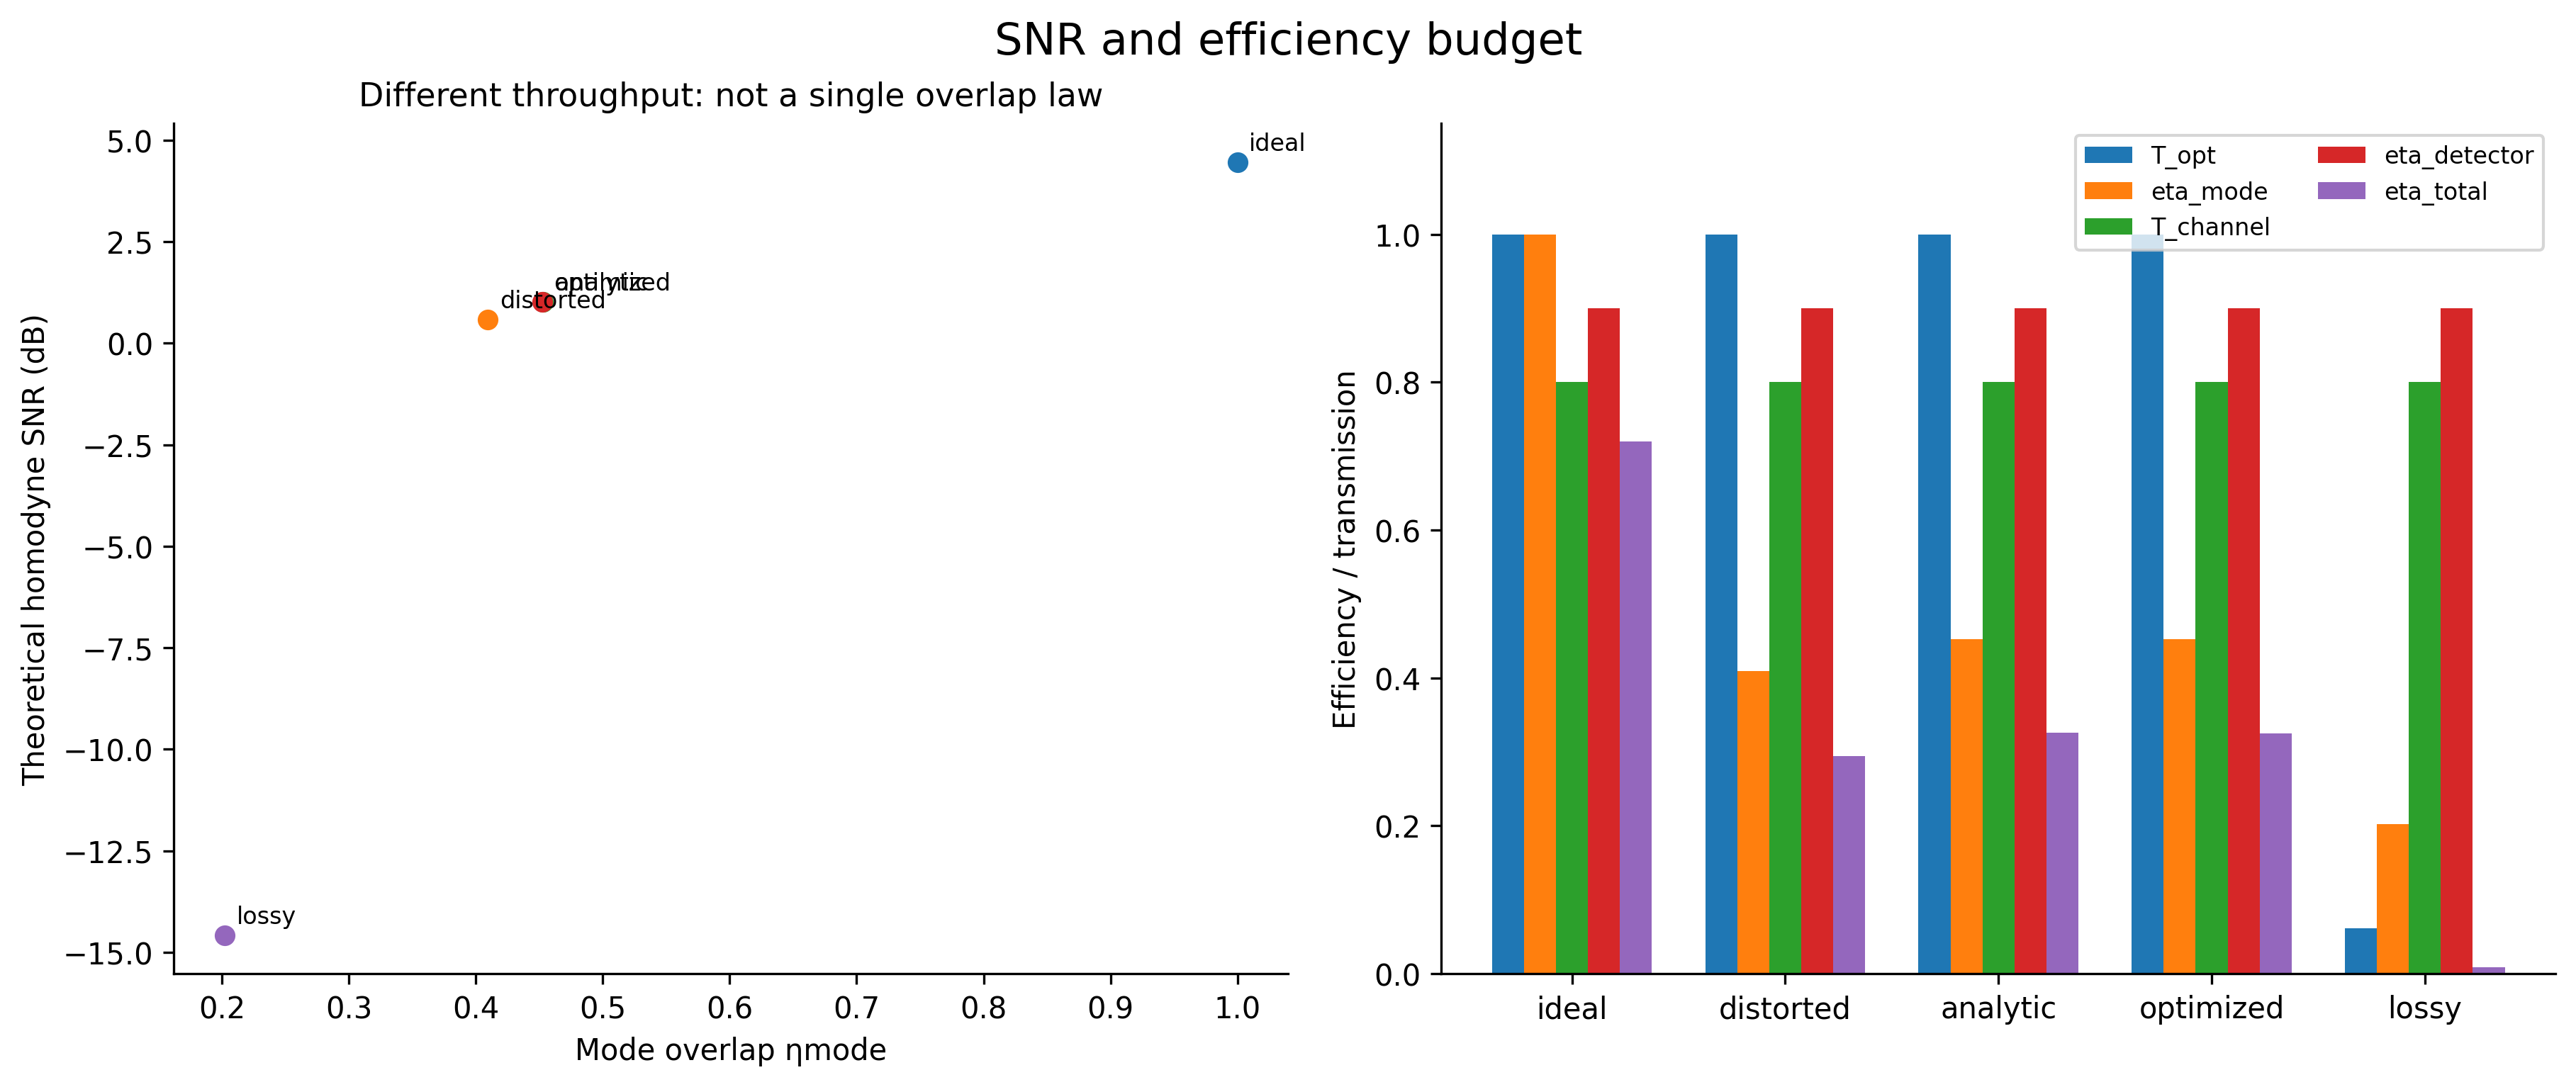
\includegraphics[width=0.94\textwidth]{../results/figures/09_snr.png}
\caption{Theoretical homodyne SNR and multiplicative efficiency budget for the representative cases. Channel transmission, optical throughput, mode overlap, and detector efficiency jointly determine useful signal efficiency. The lossy case cannot be rescued by improved overlap because most input power is irreversibly removed. The SNR plot uses theory; the archived empirical ratio is a known latent-signal/latent-noise diagnostic, not an independently inferred receiver estimate. Classical mutual information, where reported, is not a secret-key rate.}
\label{fig:snr}
\end{figure*}

The archived quantity named \texttt{snr\_empirical} is $\operatorname{Var}(\text{latent signal})/\operatorname{Var}(\text{latent noise})$. It provides a sampler diagnostic with privileged access to components, not an experimentally available estimator with a demonstrated bias or confidence interval. Figure~\ref{fig:snr} uses theoretical values only. The archive also calculates the real Gaussian-channel expression
\begin{equation}
 I(X_\theta;Y)=\tfrac12\log_2(1+\mathrm{SNR}),
\end{equation}
which is classical mutual information for the matched variable. No reconciliation efficiency, adversarial information bound, finite-size security analysis, or secret-key rate is calculated.

In the lossy case the unconditional variance approaches the noise floor because less signal remains. This is a degradation, not a quantum enhancement. Improving mode overlap increases useful signal variance and SNR while leaving the intrinsic vacuum contribution unchanged. Passive conditioning neither creates squeezing nor restores photons removed by occlusion or attenuation.

\section{Verification: Evidence and Its Boundaries}
Table~\ref{tab:verification} organizes the checks by the property actually tested. The archived test log records 41 passed tests with 14 dependency deprecation warnings; the internal specification and code reviews record no skips, including execution of the isolated backend integration test. These are local automated and engineering checks, not external peer review or experimental certification.

\begin{table*}[!t]
\caption{Verification Categories, Archived Evidence, and Interpretation Limits}
\label{tab:verification}
\centering\footnotesize
\begin{tabular}{p{0.18\textwidth}p{0.44\textwidth}p{0.30\textwidth}}
\toprule
Category & Check and evidence & What is not established\\
\midrule
FFT and physical sampling & Centered round trips, batched odd/even grids, NumPy/Torch agreement, Fourier coordinate mapping, and physical-area power conservation. & Window, pitch, padding, or aperture convergence for every distorted field.\\
Analytic optical reference & Continuous Gaussian Fourier amplitude/profile and physical width compared with the production field; profile relative-error test threshold $10^{-10}$. & Full-vector, nonparaxial, or measured lens-train accuracy.\\
Optical metrics and bounds & Power separated from normalized overlap and phase; zero-field behavior; phase-only modulus; attenuation hierarchy; analytic attainment of the spectral-magnitude ceiling. & Recovery of lost photons or arbitrary amplitude correction.\\
Actual objective and gradients & Batched pupil-normalized objective agrees with independent detector-plane computation; archived strongest-coordinate gradient error $1.68\times10^{-12}$ versus tolerance $3.00\times10^{-7}$. & Exhaustive Jacobian verification, a global optimum, or learned superiority.\\
Optimization/data discipline & Reproducible seeded runs and validation-max checkpoint selection; distinct split seeds; paired test interval and genuine conditional-array checks. & Distribution-free robustness or uncertainty from repeated training datasets.\\
TorchOptics API audit & Power error 0; normalized self-overlap error $4.44\times10^{-16}$; periodic Fresnel comparison error $4.12\times10^{-16}$ at 1 mm, zero padding factor. & Explicit two-lens propagation or an independent convergence study.\\
Homodyne statistics & Seed reproducibility, phase rotation, independent noise/calibration, excess-noise SNR, variance intervals; pure-loss tests at $T=0,0.1,0.5,1$ and $V_A=0,4$. Exact chi-square checks for residual variance. & A receiver-inferred SNR estimator, full calibration uncertainty, or security.\\
Quantum moments/backend & Actual SF Gaussian vacuum/coherent checks at 11 transmissions; 22 cases; mean error $2.22\times10^{-16}$, covariance error 0. General covariance-loss unit tests. & SF measurement trajectories, squeezed-light generation, or an optical experiment.\\
Failure handling/configuration & Missing interpreter, subprocess failure/timeout, explicit fallback identity, rejection of wrong backend physics; selected invalid inputs and duplicate split-seed checks. & Complete validation of arbitrary custom configurations or all I/O failure modes.\\
Artifact integrity/review & Internal review reports 29 manifest artifact hashes matching, finite NPZ arrays, recomputed optical powers and efficiency products; source and numerical evidence are publicly inspectable. & Independent clean-host installation, wheel-hash locking, or external review.\\
\bottomrule
\end{tabular}
\end{table*}

Several distinctions are essential. A round-trip FFT test can pass even with an incorrect physical Fourier pitch, which is why area-weighted power and analytic Gaussian references are separate checks. A generic differentiability test can pass while the training objective is wrong, which is why the actual normalized batched objective is independently evaluated. The archived finite-difference check selects its strongest-gradient coordinate, avoiding a vacuous zero-gradient comparison outside the pupil, and uses step $10^{-5}$. It is a meaningful local check, not exhaustive derivative certification.

Similarly, the auxiliary TorchOptics \texttt{ASM\_FRESNEL} audit compares propagation over 1 mm with a NumPy Fresnel transfer function under the same periodic boundary and zero-padding-factor convention. Its small relative error establishes matching discrete conventions and API usage. It does not establish that an apparatus with finite lenses, finite detector area, and different boundaries is represented to machine precision.

Quantum verification has three distinct levels: exact Gaussian identities, execution of an independent backend for their moments, and finite-sample Monte Carlo consistency. General covariance unit tests include initially squeezed covariance matrices and verify their degradation under loss. These are tests of the covariance formula, not evidence that the simulated mask produces squeezing. The main baseline inputs and quantum-backend comparisons are vacuum and coherent states.

Finally, artifact checks test persistence and internal consistency rather than scientific truth. Hash equality establishes that a file has not changed relative to its manifest. Recomputed powers establish agreement between saved fields and saved metrics. Neither operation validates the choice of distortion distribution or the physical adequacy of a scalar paraxial model. The internal review documents are useful engineering evidence precisely because these boundaries remain explicit.

\section{Reproducibility and Data Availability}
The implementation, configurations, tests, archived numerical arrays, reports, and ten PNG/SVG figure pairs are available in the public repository \cite{repository}. This paper uses the unchanged figures under \path{results/figures/}; their presentation order is 01, 02, 03, 04, 05, 06, 10, 07, 08, and 09, yielding sequential manuscript Figs.~1--10. Quantitative claims are traceable to \path{results/metrics.json}, \path{results/config.json}, \path{results/tables/cases.csv}, and \path{results/arrays/data.npz}. The phase map is additionally exported as \texttt{optimized\_phase\_rad.npy}. Arrays should be loaded with \texttt{allow\_pickle=False}.

The supplied Linux setup uses project-local Python 3.11.12 environments with exact dependency freezes. The main numerical environment pins TorchOptics 0.4.0 and CPU PyTorch 2.5.1; the separate backend environment records Strawberry Fields 0.23.0, NumPy 1.26.4, and SciPy 1.11.4. Its isolation addresses dependency compatibility rather than changing the physical model. A main-environment manifest that lists Strawberry Fields as absent is consistent with successful execution in the separate environment. Mutable online documentation is not a substitute for these version records.

From the repository root, the documented workflow is:
\begin{quote}\small\ttfamily
bash scripts/setup\_linux.sh\\
.venv/bin/python -m pytest -q\\
.venv/bin/python -m src.run \\
\hspace*{1em}--config configs/baseline.yaml \\
\hspace*{1em}--output runs/reproduction\\
python3 scripts/verify\_artifacts.py
\end{quote}
A fresh output directory preserves the published baseline. Report-only rendering uses saved arrays and preserves simulation provenance while recording rendering provenance separately. The manuscript itself does not require retraining or generation of new data.

The simulation manifest historically records a dirty revision in a parent workspace; that identifier alone is not a complete source snapshot. The standalone export documentation explains this boundary and records preservation of the numerical outputs, with publication-related path redactions in metadata/logs. The pre-manuscript repository baseline supplied for this study is commit \href{https://github.com/MADjnr/fourier-quantum-communication/tree/aaccd508e712404303ca68f56911e6365cbcefe3}{\texttt{aaccd50}}. The standalone source record and artifact hashes should be used together, rather than treating the historical simulation revision as sufficient provenance.

Version pinning and successful local execution are not proof of a clean-host reinstall on every supported machine. Dependencies are not locked with wheel hashes, and internal TorchOptics FFT imports are version-sensitive. Setup synchronizes the named local environments and can remove unlisted packages, so those environments should not be reused for unrelated work. Public visibility also does not itself grant a software license; the repository documentation states that no license has been selected.

\section{Limitations and Implications for Physical Systems}
\subsection{Physical and Statistical Scope}
The strongest numerical agreement in this work is agreement with a deliberately idealized operator model. Scalar paraxial propagation excludes polarization coupling and vectorial effects. The inverse-image convention excludes explicit lens aberrations beyond the prescribed input phase. Periodic Fourier boundaries, source renormalization, and finite sampling require a window/pitch/padding convergence study before tolerance values can be interpreted as apparatus predictions. The largest represented paraxial angle is approximately 0.06458 rad, but that coordinate extent alone is not an error estimate for the approximation.

Baseline pupil clipping is negligible for the ordinary source cases, so their unit throughput should not be read as a realistic insertion-loss budget. The deliberately lossy case exposes the effect of amplitude damage, but a single damage pattern is not a characterization of arbitrary scattering, obscuration, or turbulence. The normal distortion distribution has no empirically calibrated parameter correlations or tails. Its small training and test sets support only the stated conditional claim.

The trained phase map is high dimensional relative to the available training examples, and model selection uses a small validation set. The held-out paired intervals quantify variation across test distortions for this selected mask, not uncertainty over optimizer seeds, distribution estimation, or hardware implementation. The deterministic scan is complementary but not a substitute for statistical coverage. No per-point uncertainty bars are supplied for the quantum figure, no receiver SNR estimator interval is provided, and the displayed variance intervals omit calibration uncertainty and multiple-comparison adjustments.

\subsection{Implementation and Fabrication Boundaries}
Internal review identifies nonblocking engineering limitations outside the checked baseline: incomplete finite/type/key validation for arbitrary custom settings, nontransactional replacement of reused output directories, and limited CLI/report/interruption regression coverage. Unknown distortion keys can be ineffective rather than rejected. These facts favor fresh run directories and explicit configuration inspection, not a claim of a fully hardened general-purpose simulator.

A continuous phase array in radians does not specify a fabricated diffractive element. A computer-generated hologram would require wavelength- and material-dependent phase-depth calibration, feature-size constraints, aperture and alignment design, diffraction-efficiency accounting, and measured fabrication error. A thin-film lithium-niobate implementation would additionally require a physically justified architecture for accessing or synthesizing the Fourier transformation; a slab or star-coupler concept is not established by a bulk-relay schematic. No etch-depth values, fabricated mask, or measured transfer function are reported here.

A useful next investigation would first establish spatial sampling convergence, then evaluate additional independent distortion/training seeds, followed by quantized and feature-limited masks with measured loss and phase errors. These are proposed future studies, not results of the archived baseline. Any quantum-communication security claim would separately require a protocol, calibrated measurement model, adversarial analysis, and finite-size treatment. Better coherent SNR is not by itself a security proof.

\section{Conclusion}
An ideal sampled Fourier-plane phase mask improves coherent receiver mode matching relative to no correction under the archived displacement, tilt, defocus, and astigmatism distribution. The independent mean overlap rises from 0.431225 to 0.470226, with a positive paired improvement interval. A fixed analytic mask achieves 0.469958, and the trained-minus-analytic interval includes zero: optimization is not demonstrated to be superior.

The optical-to-statistical interpretation depends on separating throughput, normalized overlap, and quantum noise. Independent optical references, gradient checks, automated tests, and an executed Gaussian backend establish numerical consistency within that framework. Pure loss attenuates coherent means without suppressing vacuum variance. The deliberate loss case has a strict spectral-magnitude overlap ceiling and a low coupled-power ceiling even for optimal phase alignment, so neither more training nor a different phase-only mask can undo its photon loss. These results support a reproducible baseline for mode-conditioning research, while leaving experimental validation, sampling convergence, fabrication, and quantum security explicitly unresolved.

\begin{thebibliography}{9}
\bibitem{goodman}
J. W. Goodman, \emph{Introduction to Fourier Optics}, 3rd ed. Roberts and Company, 2005.
\bibitem{weedbrook}
C. Weedbrook, S. Pirandola, R. Garc\'{i}a-Patr\'{o}n, N. J. Cerf, T. C. Ralph, J. H. Shapiro, and S. Lloyd, ``Gaussian quantum information,'' \emph{Rev. Mod. Phys.}, vol. 84, pp. 621--669, 2012, doi: 10.1103/RevModPhys.84.621.
\bibitem{torchoptics}
TorchOptics, ``Official documentation.'' [Online]. Available: \url{https://torchoptics.readthedocs.io/en/latest/}
\bibitem{sfloss}
Strawberry Fields, ``LossChannel: Official API documentation.'' [Online]. Available: \url{https://strawberryfields.readthedocs.io/en/stable/code/api/strawberryfields.ops.LossChannel.html}
\bibitem{sfdocs}
Strawberry Fields, ``Official documentation.'' [Online]. Available: \url{https://strawberryfields.readthedocs.io/en/stable/}
\bibitem{repository}
A. Madu and T. Karim, ``Fourier-domain coherent communication: implementation and archived numerical evidence,'' project repository. [Online]. Available: \url{https://github.com/MADjnr/fourier-quantum-communication}
\end{thebibliography}
\end{document}
